\documentclass[oneside]{book}

\setcounter{tocdepth}{2}
\setcounter{secnumdepth}{3}

\usepackage[toc,page]{appendix}
\usepackage{minted}
\usepackage[english]{babel}
\usepackage{graphicx}
\usepackage{hyperref}
\usepackage{amsmath} % Required for some math elements 
\usepackage{pdflscape}
\usepackage{pdfpages}

\newminted[HaskellCode]{haskell}{fontsize=\footnotesize}

\begin{document}

\begin{titlepage}
	\centering
	
\includegraphics[width=0.60\textwidth]{./logo/UoN_Primary_Logo_RGB.png}\par\vspace{1cm}
	{\scshape\Large 2nd Year Report\par}
	\vspace{1.5cm}
	{\huge\bfseries Functional \\ Agent-Based Simulation\par}
	\vspace{2cm}
	{\Large Jonathan Thaler (4276122) \\ \itshape jonathan.thaler@nottingham.ac.uk \par}
	\vfill
	supervised by\par
	Dr. Peer-Olaf \textsc{Siebers} \\
	Dr. Thorsten \textsc{Altenkirch}

	\vfill

	{\large \today\par}
\end{titlepage}

\cleardoublepage

\section*{Abstract}
TODO: from the annual review i got the feedback that i need to come up with a more coherent thesis structure which tells a story: i need to make myself clear what story i want to tell with my phd and what research and publications i still need to do for that (identify chapters and to which extent they are already finished). Also I need to come up with a precise publication plan, focusing on writing papers early than doing research for a too long time and starting an early thesis writing. This is because any unpublished research is lost and every published research is a contribution to knowledge. "A good PhD is asking more questions than it answers."

This Ph.D. investigates how Agent-Based Simulations (ABS) can be implemented using the functional programming paradigm and what the benefits and drawbacks are when doing so. Due to the nature of the functional paradigm we hypothesize that by using this approach we can increase confidence in the correctness of the simulation to an unprecedented level not possible with the established object-oriented approaches in the field. The correctness of a simulation and its results is of paramount interest in scientific computing thus giving our research fundamental importance.

So far we researched \textit{how} to do ABS using the functional paradigm, where we implemented a highly promising approach by building on Functional Reactive Programming using the library Yampa and generalising it to Monadic Stream Functions. By this we could show that ABS is indeed very possible in functional programming as it allowed us to implement a number of different agent-based models, incorporating discrete time-semantics similar to Discrete Event Simulation and continuous time-flows like System Dynamics.

During the research conducted so far, it became apparent that this approach exhibits a few unique properties which indeed supports our initial hypothesis. We have started to systematically explore these properties through the additional use of dependent types and will commit our research of the next 8 months to fully develop this. We expect that dependent types allow us to narrow the gap between model specification and implementation on an unprecedented level, implying by definition, that a simulation is correct-by-construction.

\clearpage
\tableofcontents
\clearpage

\section{Introduction}
There exists a large number of simulation packages which allow the convenient creation of System Dynamics simulations by straight-forward visual diagram creation. One simply creates stocks and flows, connects them, specifies the flow-rates and initial parameters and then runs the model. An example for such a visual diagram creation in the simulation package AnyLogic can be seen in Figure \ref{fig:sir_stockflow_diagram}.

\begin{figure}
	\centering
	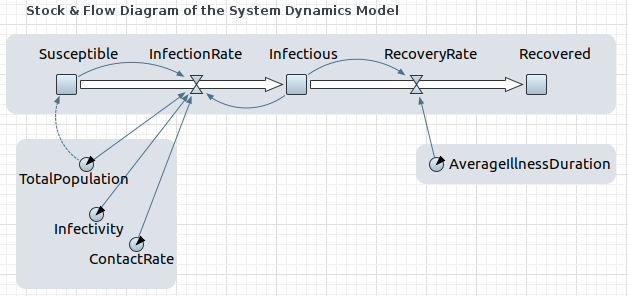
\includegraphics[width=.5\textwidth, angle=0]{./fig/SIR_SD_STOCKFLOW_DIAGRAMM.png}
	\caption{Visual System Dynamics Diagram of the SIR model in AnyLogic Personal Learning Edition 8.3.1.}
	\label{fig:sir_stockflow_diagram}
\end{figure}

Still, implementing System Dynamics directly in code is not as straight forward and involves numerical integration which can be quite tricky to get right. Thus, the aim of this paper is to look into how System Dynamics models can be implemented in code correctly without the use of a simulation package. We use the well known SIR model \cite{kermack_contribution_1927} from epidemiology to demonstrate our approach.

Our language of choice is Haskell because it emphasises a declarative programming style in which one describes \textit{what} instead of \textit{how} to compute. Further it allows to rule out interference with non-deterministic influences or side-effects already at compile-time. This is of fundamental importance for System Dynamics because it behaves completely deterministic and involves no stochastics or non-determinism whatsoever. Also, we make use of Functional Reactive Programming which allows to express continuous-time systems in a functional way. 

We show that by this approach we can arrive at correct-by-construction implementations of System Dynamic models. This means that the correctness of the code is obvious because we have closed the gap between the model specification and its implementation. Thus, the contribution of the paper is the demonstration of how to implement correct-by-construction System Dynamics simulations using Haskell and Functional Reactive Programming.

\section{Software Transactional Memory}
Software Transactional Memory was introduced by \cite{shavit_software_1995} in 1995 as an alternative to lock-based synchronisation in concurrent programming which, in general, is notoriously difficult to get right. This is because reasoning about the interactions of multiple concurrently running threads and low level operational details of synchronisation primitives is \textit{very hard}. The main problems are \cite{marlow_parallel_2013}:

\begin{itemize}
	\item Race conditions due to forgotten locks;
	\item Deadlocks resulting from inconsistent lock ordering;
	\item Corruption caused by uncaught exceptions;
	\item Lost wake-ups induced by omitted notifications.
\end{itemize}

What is worse, concurrency does not compose. It is very difficult to write two functions (or methods in an object) acting on concurrent data which can be composed into a larger concurrent behaviour. The reason for the difficulty is that one has to know about the internal details of locking, which breaks encapsulation and makes composition dependent on knowledge about their implementation. Therefore, it is impossible to compose two functions where, for example, one withdraws some amount of money from an account and the other deposits this amount of money into a different account. The problem is that one ends up with a temporary state where the money is in neither of the accounts, creating an inconsistency and a potential source for errors because threads can be rescheduled at any time.

STM promises to solve all of these problems for a low cost by executing actions \textit{atomically}, where modifications made in such an action are invisible to other threads and changes by other threads are also invisible until actions are committed - STM actions are atomic and isolated. When an STM action exits, either one of two outcomes happen: if no other thread has modified the same data as the thread running the STM action, then the modifications performed by the action will be committed and become visible to the other threads. If other threads have modified the data then the modifications will be discarded, the action rolled back and automatically restarted.

\subsection{Software Transactional Memory in Haskell}
The work of \cite{harris_composable_2005, harris_transactional_2006} added STM to Haskell, which was one of the first programming languages to incorporate STM with composable operations into its main core. In the Haskell implementation, STM actions run within the \texttt{STM} Monad. This restricts the operations to only STM primitives as shown below. This means that \texttt{STM} actions are always repeatable without persistent side effects because such persistent side effects (for example writing to a file, launching a missile) are not possible in the \texttt{STM} Monad. This is also the fundamental difference to \texttt{IO}, where all bets are off and \textit{everything} is possible because \texttt{IO} can run everything without restrictions.

Thus, the ability to \textit{restart} an action without any persistent effects is only possible due to the nature of Haskell's type system and by restricting the effects to \texttt{STM} only, ensures that only controlled effects, which can be rolled back, occur.

STM comes with a number of primitives to share transactional data. Amongst others the most important ones are:

\begin{itemize}
	\item \texttt{TVar} - a transactional variable which can be read and written arbitrarily;
	
	\item \texttt{TMVar} - a transactional \textit{synchronising} variable which is either empty or full. To read from an empty or write to a full \texttt{TMVar} will cause the current thread to block and retry its transaction when \textit{any} transactional primitive of this action has changed.
	
	\item \texttt{TArray} - a transactional array where each cell is an individual transactional variable \texttt{TVar}, allowing more finer-grained transactions instead of having the whole array in a \texttt{TVar}.
	
	\item \texttt{TChan} - a transactional channel, representing an unbounded FIFO channel, based on a linked list of \texttt{TVar}.
\end{itemize}

Furthermore STM also provides combinators to deal with blocking and composition:

\begin{itemize}
	\item \texttt{retry :: STM ()} retries an \texttt{STM} action. This will cause to abort the current transaction and block the thread it is running in. When \textit{any} of the transactional data primitives have changed, the action will be run again. This is useful to await the arrival of data in a \texttt{TVar}, or put more general, to block on arbitrary conditions. 
	
	\item \texttt{orElse :: STM a $\rightarrow$ STM a $\rightarrow$ STM a} allows us to combine two blocking actions where either one is executed, but not both. The first action is run and if it is successful its result is returned. If it retries, then the second is run and if that one is successful its result is returned. If the second one retries, the whole \texttt{orElse} retries. This can be used to implement alternatives in blocking conditions, which can obviously be nested arbitrarily.
\end{itemize}

To run an \texttt{STM} action the function \texttt{atomically :: STM a $\rightarrow$ IO a} is provided, which performs a series of \texttt{STM} actions atomically within the \texttt{IO} Monad. It takes the \texttt{STM} action, which returns a value of type \texttt{a} and returns an \texttt{IO} action which returns a value of type \texttt{a}. The \texttt{IO} action then can only be executed from within the \texttt{IO} Monad, either within the main thread or an explicitly forked thread.

STM in Haskell is implemented using optimistic synchronisation, which means that instead of locking access to shared data, each thread keeps a transaction log for each read and write to shared data that it makes. When the transaction exits, the thread checks whether it has a consistent view to the shared data or not. It checks whether other threads have written to memory it has read, thus it can identify whether a rollback is required or not.

However, STM does not come without issues. The authors of \cite{perfumo_limits_2008} analyse several Haskell STM programs with respect to their transactional behaviour. They identified the roll-back rate as one of the key metrics, which determines the scalability of an application. Although STM might promise better performance, they also warn of the overhead it introduces, which could be quite substantial in particular for programs which do not perform much work inside transactions as their commit overhead is high.

\subsection{STM Examples}
We provide two examples to demonstrate the use and semantics of STM. The first example is an implementation of the aforementioned functionality, where money is withdrawn from one account and transferred to another. The implementing function \texttt{transferFunds} takes two \texttt{TVar}, holding the account balances, and the amount to exchange. It executes using \texttt{atomically}, therefore running in the \texttt{IO} Monad. It uses the two functions \texttt{withdraw} and \texttt{deposit} which do the work of withdrawing some amount from one account and depositing some amount to another. This example demonstrates how easily STM can be used: the implementation looks quite straightforward, simply swapping values, without any locking involved or special handling of concurrency, other than the use of \texttt{atomically}.

\begin{HaskellCode}
transferFunds :: TVar Integer -> TVar Integer -> Integer -> IO ()
transferFunds from to n = atomically (do
  withdraw from n
  deposit to n)
  
withdraw :: TVar Integer -> Integer -> STM ()
withdraw account amount = do
  balance <- readTVar account
  writeTVar (balance - amount)
  
deposit :: TVar Integer -> Integer -> STM ()
deposit account amount = do
  balance <- readTVar account
  writeTVar (balance + amount)
\end{HaskellCode}

In the second example we show the retry semantics of STM, by using it within a \texttt{StateT} transformer where \texttt{STM} is the innermost Monad. It is important to understand that \texttt{STM} does not provide a transformer instance for very good reasons. If it would provide a transformer then we could make \texttt{IO} the innermost Monad and perform \texttt{IO} actions within \texttt{STM}. This would violate the retry semantics, as in case of a retry, \texttt{STM} is unable to undo the effects of \texttt{IO} actions in general. This stems from the fact that the \texttt{IO} type is simply too powerful and we cannot distinguish between different kinds of \texttt{IO} actions in the type, be it simply reading from a file or actually launching a missile. Let's look at the example code:

\begin{HaskellCode}
stmAction :: TVar Int -> StateT Int STM Int 
stmAction v = do
  -- print a debug output and increment the value in StateT 
  Debug.trace "increment!" (modify (+1))
  -- read from the TVar
  n <- lift (readTVar v)
  -- await a condition: content of the TVar >= 42
  if n < 42
    -- condition not met: retry
    then lift retry
    -- condition met: return content ot TVar
    else return n
\end{HaskellCode}

In this example, the \texttt{STM} is the innermost Monad in a stack with a \texttt{StateT} transformer. When \texttt{stmAction} is run, it prints an \texttt{'increment!'} debug message to the console and increments the value in the \texttt{StateT} transformer. Then it awaits a condition. For as long as \texttt{TVar} is less then 42 the action will retry whenever it is run. If the condition is met, it will return the content of the \texttt{TVar}. We see the combined effects of using the transformer stack where we have both the \texttt{StateT} and the \texttt{STM} effects available. The question is how this code behaves if we actually run it. To do this we need to spawn a thread:

\begin{HaskellCode}
stmThread :: TVar Int -> IO ()
stmThread v = do
  -- the initial state of the StateT transformer
  let s = 0
  -- run the state transformer with initial value of s (0)
  let ret = runStateT (stmAction v) s
  -- atomically run the STM block
  (a, s') <- atomically ret
  -- print final result
  putStrLn("final StateT state     = " ++ show s' ++
           ", STM computation result = " ++ show a)
\end{HaskellCode}

The thread simply runs the \texttt{StateT} transformer layer with the initial value of 0 and then the \texttt{STM} computation through \texttt{atomically} and prints the result to the console. The value of \texttt{a} is the result of \texttt{stmAction} and \texttt{s'} is the final state of the \texttt{StateT} computation. To actually run this example we need the main thread to update the \texttt{TVar} until the condition is met within \texttt{stmAction}:

\begin{HaskellCode}
main :: IO ()
main = do
  -- create a new TVar with initial value of 0
  v <- newTVarIO 0 
  -- start the stmThread and pass the TVar
  forkIO (stmThread v)
  -- do 42 times...
  forM_ [1..42] (\i -> do
    -- use delay to 'make sure' that a retry is happening for ever increment
    threadDelay 10000
    -- write new value to TVar using atomically
    atomically (writeTVar v i))
\end{HaskellCode}

If we run this program, we will see \texttt{'increment!'} printed 43 times, followed by \texttt{'final StateT state = 1, STM computation result = 42'}. This clearly demonstrates the retry semantics where \texttt{stmAction} is retried 42 times and thus prints \texttt{'increment!'} 43 times to the console. The \texttt{StateT} computation, however, is carried out only once and is always rolled back when a retry is happening. The rollback is easily possible in pure functional programming due to persistent data structure, by simply throwing away the new value and retrying with the original value. This example also demonstrates that any \texttt{IO} actions which happen within an \texttt{STM} action are persistent and can obviously not be rolled back. \texttt{Debug.trace} is an \texttt{IO} action masked as pure using \texttt{unsafePerformIO}.

\chapter{Verification \& Validation}
\label{chap:v_and_v}

In this chapter we will have a closer look on the topic of Verification \& Validation. It is of most importance to understand the ideas and concepts behind it, when we are referring to the \textit{correctness of a simulation}, as in our initial hypothesis. 

We first will give a short and concise introduction (\ref{sec:vav_introduction}) on the topic \footnote{In this short introduction we closely follow the book \cite{robinson_simulation:_2014}} and then briefly discuss verification \& validation in the context of agent-based simulation (\ref{sec:vav_abs}).

%TODO: we need to distinguish between various meanings of 'correct'
%1. correctness of software: the implementation is correct up to a model specification
%2. correctness of a simulation: the implementation is correct up to a model specification AND it generates the same dynamics

\section{Introduction}
\label{sec:vav_introduction}
%According to \cite{robinson_simulation:_2014}, when implementing a model one should have the following aims in mind:
%\begin{itemize}
%	\item Speed Of Coding - how quickly can we implement a model.
%	\item Transparency - how easily can the code be understood.
%	\item Flexibility - how easily can the code be changed to model changes.
%	\item Run-Speed - how quickly will the code execute.
%\end{itemize}
%
%Further the author distinguishes three activities 
%\begin{itemize}
%	\item Coding - implementing the model.
%	\item Testing - verifying and white-box validating the model.
%	\item Documenting - recording details of the model.
%\end{itemize}
%
%Also it is important to distinguish between different natures of a simulation: terminating or non-terminating, and its output transient or steady-state (cycle or shifting).

%steward robinson simulation book on implementation
%- meaning of implementation
%	-> 1 implementing the findings: conduct a study which defines and gathers all findings about the model and document them
%	-> 2 implementing the model
%	-> 3 implementing the learning

\textbf{\textit{Validation}} is the process of ensuring that a model or specification is sufficiently accurate for the purpose at hand.

\textbf{\textit{Verification}} is the process of ensuring that the model design has been transformed into a computer model with sufficient accuracy.

\cite{balci_verification_1998} define validation as "are we building the right model?" and verification as "are we building the model right?".

In verification and validation the aim is to ensure, that the model is sufficiently accurate, which always implies its purpose. Therefore the purpose and objectives must be known before it is validated. 

In this research we will primarily focus on verification, because its there where one ensures that the model is programmed correctly, the algorithms have been implemented properly, and the model does not contain errors, oversights, or bugs. Note that verification has a narrow definition and can be seen as a subset of the wider issue of validation. One distinguishes between:

\begin{itemize}
	\item White-box Validation: detailed, micro check if each part of the model represent the real world with sufficient accuracy. It is therefore intrinsic to model coding. The ways to do it is checking the code, visual checks, inspecting output reports. 
	\item Black-box Validation: overall macro check whether the model provides a sufficiently accurate representation of the real world system. It can only be performed once model code is complete. Ways to do this is comparison with the real system or with other (simpler) models.

	\item White-box Verification: compares the content of the model to the \textit{conceptual} model. This is different to white-box validation which compares the content of the model to the \textit{real world}
	\item Black-box Verification: treating the functionality to test as a black-box with inputs and outputs and comparing controlled inputs to expected outputs.

	%\item Data Validation: determining that the contextual data and the data required for model realisation and validation are sufficiently accurate for the purpose at hand.
\end{itemize}

%good paper \url{http://www2.econ.iastate.edu/tesfatsi/VVAccreditationSimModels.OBalci1998.pdf} : very nice 15 guidelines and life cycles, VERY valuable for background and introduction

So in general one can see verification as a test of the fidelity with which the conceptual model is converted into the computer model. Verification (and validation) is a continuous process and if it is already there in the programming language / supported by then this is much easier to do. This is the fundamental basis of our hypothesis where we claim that by choosing a programming language which supports this continuous verification and validation process, then the result is an implementation of a model which is more likely to be correct.

Unfortunately, there is no such thing as general validity: a model should be built for one purpose as simple as possible and not be too general, otherwise it becomes too bloated and too difficult or impossible to analyse. Also, there may be no real world to compare against: simulations are developed for proposed systems, new production or facilities which don't exist yet. Further, it is questionable which real world one is speaking of: the real world can be interpreted in different ways, therefore a model valid to one person might not be valid to another. Sometimes validation struggles because the real world data are inaccurate or there is not enough time to verify and validate everything.

In general this implies that we can only \textit{raise the confidence} in the correctness of the simulation: it is not possible to prove that a model is valid, instead one should think of confidence in its validity. Therefore, the process of verification and validation is not the proof that a model is correct but trying to prove that the model is incorrect! The more tests/checks one carries out which show that it is not incorrect, the more confidence we can place on the models validity.

%	- methods of verification and validation
%	-> conceptual model validation: judment based on the documentation
%	-> data validation: analysing data for inconsistencies
%	-> verification and white-box validation
%		-> both conceptually different but often treated together because both occur continuously through model coding
%		-> what should be checked: timings (cycle times, arrival times,...), control of elements (breakdown frequency, shift patterns), control flows (e.g. routing), control logic (e.g. scheduling, stock replenishment), distribution sampling (samples obtained from an empirial distribution)
%	-> verification and whilte-box validation methods
%		-> checking code: reading through code and ensure right data and logic is there. explain to others/discuss together/others should look at your code. 
%		-> Visual checks
%		-> inspecting output reports
%		
%	-> black-box testing: consider overall behaviour of the model without looking into its parts, basically two ways
%		-> comparison with the real system: statistical tests
%		-> comparison with another model (e.g. mathematical equations): could compare exactly or also through statistical tests
%		-> 
%		

%peers slides (inspired by steward robinson book):
%    - Experimentation Validation: Determining that the experimental procedures adopted are providing results that are sufficiently accurate for the purpose at hand.
%    	-> How can we do this?
%    		- Graphical or statistical methods for determining warm-up period, run length and replications (to obtain accurate results)
%			- Sensitivity analysis (to improve the understanding of the model)
%	
%	- Solution Validation: Determining that the results obtained from the model of the proposed solution are sufficiently accurate for the purpose at hand
%		-> How does this differ from Black Box Validation? Solution validation compares the model of the proposed solution to the implemented solution while black-box validation compares the base model to the real world
%		-> How can we do this? Once implemented it should be possible to validate the implemented solution against the model results
%		
%	- Verification: Testing the fidelity with which the conceptual model is converted into the computer model. Verification is done to ensure that the model is programmed correctly, the algorithms have been implemented properly, and the model does not contain errors, oversights, or bugs.
%
%		-> How can we do this? Same methods as for white-box validation (checking the code, visual checks, inspecting output reports) but ... Verification compares the content of the model to the conceptual model while white-box validation compares the content of the model to the real world
%		
%	- Difficulties of verification and validation
%		-> There is no such thing as general validity: a model is only valid with respect to its purpose
%		-> There may be no real world to compare against
%		-> Which real world? Different people have different interpretations of the real world
%		->  Often real world data are inaccurate: If the data are not accurate it is difficult to determine if the model's results are correct. Even if the data is accurate, the real worl  data are only a sample, which in itself creates inaccuracy
%		-> There is not enough time to verify and validate every aspect of a model
%		
%	- Some final remarks:
%		-> V\&V is a continuous and iterative process that is performed throughout the life cycle of a simulation study.
%			Example: If the conceptual model is revised as the project progresses it needs to be re-validated
%		-> V\&V work together by removing barriers and objections to model use and hence establishing credibility.
%		
%- Conclusion: Although, in theory, a model is either valid or not, proving this in practice is a very different matter. It is better to think in terms of confidence that can be placed in a model!

\section{Verification \& Validation in Agent-Based Simulation}
\label{sec:vav_abs}
In our research we focus primarily on the \textit{Verification} aspect of agent-based simulation: ensuring that the implementation reflects the specifications of the \textit{conceptual} model - have we built the model right? Thus we are not interested in our research into making connections to the real world and always see the model specifications as our "last resort", our ground truth beyond nothing else exists. When there are hypotheses formulated, we always treat and interpret them in respect of the conceptual model.

In \cite{ormerod_validation_2006} the authors clarify on verification in ABS. Verification "... is essentially the question: does the model do what we think it is supposed to do? Whenever a model has an analytical solution, a condition which embraces almost all conventional economic theory, verification is a matter of checking the mathematics.". They say about validation that "In an important sense, the current process of building ABMs is a discovery process, of discovering the types of behavioural rules for agents which appear to be consistent with phenomena we observe.". Further they claim that "Because such models are based on simulation, the lack of an analytical solution (in general) means that verification is harder, since there is no single result the model must match. Moreover, testing the range of model outcomes provides a test only in respect to a prior judgment on the plausibility of the potential range of outcomes. In this sense, verification blends into validation."

So the baseline is that either one has an analytical model as the basis of an agent-based model or one does not. In the former case, e.g. the SIR model, one can very easily validate the dynamics generated by the simulation to the one generated by the analytical solution (e.g. through System Dynamics). In the latter case one has basically no idea or description of the emergent behaviour of the system prior to its execution e.g. SugarScape. It is important to have some hypothesis about the emergent property / dynamics. The question is how verification / validation works in this setting as there is no formal description of the expected behaviour: we don't have a ground-truth against which we can compare our simulation dynamics. %(eventuell hilft hier hans vollbrecht weiter: Simulation hat hier den Sinn, die Controller anhand der Roboteraufgabe zu validieren, Bei solchen Simulationen ist man interessiert an allen möglichen Sequenzen, und da das meist zu viele sind, an einer möglichst gut verteilten Stichprobenmenge. Hier geht es weniger um richtige Zeitmodellierung, sondern um den Test aller möglichen Ereignissequenzen.)

General there are the following basic verification \& validation requirements to ABS \cite{robinson_simulation:_2014}, which all can be addressed in our \textit{pure} functional approach as described in the paper in Appendix \ref{app:pfe}:

\begin{itemize}
	%\item Modelling progress of time - achieved using functional reactive programming (FRP)
	%\item Modelling variability - achieved using FRP
	\item Fixing random number streams to allow simulations to be repeated under same conditions - ensured by \textit{pure} functional programming and Random Monads
	\item Rely only on past - guaranteed with \textit{Arrowized} FRP
	\item Bugs due to implicitly mutable state - reduced using pure functional programming
	\item Ruling out external sources of non-determinism / randomness - ensured by \textit{pure} functional programming
	\item Deterministic time-delta - ensured by \textit{pure} functional programming
	\item Repeated runs lead to same dynamics - ensured by \textit{pure} functional programming
\end{itemize}

\subsection{Related Work}
The work of \cite{kleijnen_verification_1995} suggests good programming practice which is extremely important for high quality code and reduces bugs but real world practice and experience shows that this alone is not enough, even the best programmers make mistakes which often can be prevented through a strong static or a dependent type system already at compile-time. What we can guarantee already at compile-time, doesn't need to be checked at run-time which saves substantial amount of time as at run-time there may be a large number of execution paths through the simulation which is almost always simply not feasible to check (note that we also need to check all combinations). This paper also cites modularity as very important for verification: divide and conquer and test all modules separately. We claim that this is especially easy in functional programming as code composes better than in traditional object-oriented programming due to the lack of interdependence between data and code as in objects and the lack of global mutable state (e.g. class variables or global variables) - this makes code extremely convenient to test. The paper also discusses statistical tests (the t test) to check if the outcome of a simulation is sufficiently close to real-world dynamics - we explicitly omit this as it part of validation and not the focus of this research. % Also the paper suggests using animations to visualise the processes within the simulation for verification purposes (of course they note that animation may be misleading when one focuses on too short simulation runs).

%So we ask whether we can encode phenomena we observe in the types? can we use types for the discovery process as well? can dependent types guide our exploratory approach to ABS?

\cite{polhill_ghost_2005}: \textit{"For some time now, Agent Based Modelling has been used to simulate and explore complex systems, which have proved intractable to other modelling approaches such as mathematical modelling. More generally, computer modelling offers a greater flexibility and scope to represent phenomena that do not naturally translate into an analytical framework. Agent Based Models however, by their very nature, require more rigorous programming standards than other computer simulations. This is because researchers are cued to expect the unexpected in the output of their simulations: they are looking for the 'surprise' that shows an interesting emergent effect in the complex system. It is important, then, to be absolutely clear that the model running in the computer is behaving exactly as specified in the design. It is very easy, in the several thousand lines of code that are involved in programming an Agent Based Model, for bugs to creep in. Unlike mathematical models, where the derivations are open to scrutiny in the publication of the work, the code used for an Agent Based Model is not checked as part of the peer-review process, and there may even be Intellectual Property Rights issues with providing the source code in an accompanying web page."}

\cite{galan_errors_2009}: \textit{"a prerequisite to understanding a simulation is to make sure that there is no significant disparity between what we think the computer code is doing and what is actually doing. One could be tempted to think that, given that the code has been programmed by someone, surely there is always at least one person - the programmer - who knows precisely what the code does. Unfortunately, the truth tends to be quite different, as the leading figures in the field report, including the following: You should assume that, no matter how carefully you have designed and built your simulation, it will contain bugs (code that does something different to what you wanted and expected), "Achieving internal validity is harder than it might seem. The problem is knowing whether an unexpected result is a reflection of a mistake in the programming, or a surprising consequence of the model itself. […] As is often the case, confirming that the model was correctly programmed was substantially more work than programming the model in the first place. This problem is particularly acute in the case of agent-based simulation. The complex and exploratory nature of most agent-based models implies that, before running a model, there is some uncertainty about what the model will produce. Not knowing a priori what to expect makes it difficult to discern whether an unexpected outcome has been generated as a legitimate result of the assumptions embedded in the model or, on the contrary, it is due to an error or an artefact created in the model design, its implementation, or its execution."}

\subsection{Testing}
Although (pure) functional programming allows us to have stronger guarantees about the behaviour and absence of bugs of the simulation already at compile-time, we still need to test all the properties of our simulation which we cannot guarantee at compile-time.

We found property-based testing particularly well suited for ABS. Although it is now available in a wide range of programming languages and paradigms, propert-based testing has its origins in Haskell \cite{claessen_quickcheck:_2000, claessen_testing_2002} and we argue that for that reason it really shines in pure functional programming. Property-based testing allows to formulate \textit{functional specifications} in code which then the property-testing library (e.g. QuickCheck \cite{claessen_quickcheck:_2000}) tries to falsify by automatically generating random test-data covering as much cases as possible. When an input is found for which the property fails, the library then reduces it to the most simple one. It is clear to see that this kind of testing is especially suited to ABS, because we can formulate specifications, meaning we describe \textit{what} to test instead of \textit{how} to test (again the declarative nature of functional programming shines through). Also the deductive nature of falsification in property-based testing suits very well the constructive nature of ABS.

Generally we need to distinguish between two types of testing/verification: 1. testing/verification of models for which we have real-world data or an analytical solution which can act as a ground-truth - examples for such models are the SIR model, stock-market simulations, social simulations of all kind and 2. testing/verification of models which are just exploratory and which are only be inspired by real-world phenomena - examples for such models are Epsteins Sugarscape and Agent\_Zero.

In both cases this leaves us with black-box and white-box Verification:

%\subsection{Comparison of dynamics against existing data}
%- utilise a statistical test with H0 "ABS and comparison is not the same" and H1 "ABS and comparison is the same"
%- how many replications and how do we average?
%- which statistical test do we implement? (steward robinson simulation book, chapter 12.4.4)
%	-> Normalizsed Mean Squared Error (NMSE)
%	-> TODO: implement confidence interval 
%	-> TODO: what about chi-squared?
%	-> TODO: what about paired-t confidence interval
%
%IMPORTANT: this is not what we are after here in this paper, statistical tests are a science on their own and there actually exists quite a large amount of literature for conducting statistical tests on ABS dynamics: Robinson Book (TODO: find additional literature)	

\subsubsection{Black-Box Verification}
In black-box Verification one generally feeds input and compares it to expected output. In the case of ABS we have the following examples of black-box test:
\begin{enumerate}
	\item Isolated Agent Behaviour - test isolated agent behaviour under given inputs using and property-based testing.
	\item Interacting Agent Behaviour - test if interaction between agents are correct .
	\item Simulation Dynamics - compare emergent dynamics of the ABS as a whole under given inputs to an analytical solution or real-world dynamics in case there exists some using statistical tests.
	\item Hypotheses- test whether hypotheses are valid or invalid using and property-based testing. % TODO: how can we formulate hypotheses in unit- and/or property-based tests?
\end{enumerate}

%- testing of the final dynamics: how close do they match the analytical solution
%- can we express model properties in tests e.g. quickcheck?
%- property-testing shines here
%- isolated tests: how easy can we test parts of an agent / simulation?

Using black-box verification and property-based testing we can apply for the following use cases for testing ABS in FRP:

\paragraph{Finding optimal $\Delta t$}
The selection of the right $\Delta t$ can be quite difficult in FRP because we have to make assumptions about the system a priori. One could just play it safe with a very conservative, small $\Delta t < 0.1$ but the smaller $\Delta t$, the lower the performance as it multiplies the number of steps to calculate. Obviously one wants to select the \textit{optimal} $\Delta t$, which in the case of ABS is the largest possible $\Delta t$ for which we still get the correct simulation dynamics.
To find out the \textit{optimal} $\Delta t$ one can make direct use of the black-box tests: start with a large $\Delta t = 1.0$ and reduce it by half every time the tests fail until no more tests fail - if for $\Delta t = 1.0$ tests already pass, increasing it may be an option. It is important to note that although isolated agent behaviour tests might result in larger $\Delta t$, in the end when they are run in the aggregate system, one needs to sample the whole system with the smallest $\Delta t$ found amongst all tests. Another option would be to apply super-sampling to just the parts which need a very small $\Delta t$ but this is out of scope of this paper.

\paragraph{Agents as signals}
Agents \textit{might} behave as signals in FRP which means that their behaviour is completely determined by the passing of time: they only change when time changes thus if they are a signal they should stay constant if time stays constant. This means that they should not change in case one is sampling the system with $\Delta t = 0$. Of course to prove whether this will \textit{always} be the case is strictly speaking impossible with a black-box verification but we can gain a good level of confidence with them also because we are staying pure. It is only through white-box verification that we can really guarantee and prove this property.

\subsubsection{White-Box Verification}
White-Box verification is necessary when we need to reason about properties like \textit{forever}, \textit{never}, which cannot be guaranteed from black-box tests. Additional help can be coverage tests with which we can show that all code paths have been covered in our tests.

\subsection{Example: Property-Based Testing of SIR}
As an example we discuss the black-box testing for the SIR model using property-testing. We test if the \textit{isolated} behaviour of an agent in all three states Susceptible, Infected and Recovered, corresponds to model specifications. The crucial thing though is that we are dealing with a stochastic system where the agents act \textit{on averages}, which means we need to average our tests as well. We conducted the tests on the implementation found in the paper of Appendix \ref{app:pfe}.

\subsubsection{Black-Box Verification}
The interface of the agent behaviours are defined below. When running the SF with a given $\Delta t$ one has to feed in the state of all the other agents as input and the agent outputs its state it is after this $\Delta t$.

\begin{HaskellCode}
data SIRState 
  = Susceptible 
  | Infected 
  | Recovered
  
type SIRAgent = SF [SIRState] SIRState

susceptibleAgent :: RandomGen g => g -> SIRAgent
infectedAgent :: RandomGen g => g -> SIRAgent
recoveredAgent :: SIRAgent
\end{HaskellCode}

\paragraph{Susceptible Behaviour}
A susceptible agent \textit{may} become infected, depending on the number of infected agents in relation to non-infected the susceptible agent has contact to. To make this property testable we run a susceptible agent for 1.0 time-unit (note that we are sampling the system with a smaller $\Delta t = 0.1$) and then check if it is infected - that is it returns infected as its current state.

Obviously we need to pay attention to the fact that we are dealing with a stochastic system thus we can only talk about averages and thus it does not suffice to only run a single agent but we are repeating this for e.g. $N = 10.000$ agents (all with different RNGs). We then need a formula for the required fraction of the N agents which should have become infected on average. Per 1.0 time-unit, a susceptible agent makes \textit{on average} contact with $\beta$ other agents where in the case of a contact with an infected agent the susceptible agent becomes infected with a given probability $\gamma$. In this description there is another probability hidden, which is the probability of making contact with an infected agent which is simply the ratio of number of infected agents to number not infected agents. The formula for the target fraction of agents which become infected is then: $\beta * \gamma * \frac{number of infected}{number of non-infected}$. To check whether this test has passed we compare the required amount of agents which on average should become infected to the one from our tests (simply count the agents which got infected and divide by N) and if the value lies within some small $\epsilon$ then we accept the test as passed.

Obviously the input to the susceptible agents which we can vary is the set of agents with which the susceptible agents make contact with. To save us from constructing all possible edge-cases and combinations and testing them with unit-tests we use property-testing with QuickCheck which creates them randomly for us and reduces them also to all relevant edge-cases. This is an example for how to use property-based testing in ABS where QuickCheck can be of immense help generating random test-data to cover all cases.

%TODO: derive the target-fraction formula from the differential equations
%TODO: can we encode this somehow on a type level using dependent types? then we don't need to test this property any more

\paragraph{Infected Behaviour}
An infected agent \textit{will always} recover after a finite time, which is \textit{on average} after $\delta$ time-units. Note that this property involves stochastics too, so to test this property we run a large number of infected agents e.g. $N = 10.000$ (all with different RNGs) until they recover, record the time of each agents recovery and then average over all recovery times. To check whether this test has passed we compare the average recovery times to $\delta$ and if they lie within some small $\epsilon$ then we accept the test as passed.

We use property-testing with QuickCheck in this case as well to generate the set of other agents as input for the infected agents. Strictly speaking this would not be necessary as an infected agent never makes contact with other agents and simply ignores them - we could as well just feed in an empty list. We opted for using QuickCheck for the following reasons:

\begin{itemize}
	\item We wanted to stick to the interface specification of the agent-implementation as close as possible which asks to pass the states of all agents as input.
	\item We shouldn't make any assumptions about the actual implementation and if it REALLY ignores the other agents, so we strictly stick to the interface which requires us to input the states of all the other agents.
	\item The set of other agents is ignored when determining whether the test has failed or not which indicates by construction that the behaviour of an infected agent does not depend on other agents.
	\item We are not just running a single replication over 10.000 agents but 100 of them which should give black-box verification more strength.
\end{itemize}

%TODO: derive the average formula from the differential equations
%TODO: can we encode this somehow on a type level using dependent types? then we don't need to test this property any more

\paragraph{Recovered Behaviour}
A recovered agent will stay in the recovered state \textit{forever}. Obviously we cannot write a black-box test that truly verifies that because it had to run in fact forever. In this case we need to resort to white-box verification (see below).

Because we use multiple replications in combination with QuickCheck obviously results in longer test-runs (about 5 minutes on my machine)
In our implementation we utilized the FRP paradigm. It seems that functional programming and FRP allow extremely easy testing of individual agent behaviour because FP and FRP compose extremely well which in turn means that there are no global dependencies as e.g. in OOP where we have to be very careful to clean up the system after each test - this is not an issue at all in our \textit{pure} approach to ABS.

\paragraph{Simulation Dynamics}
We won't go into the details of comparing the dynamics of an ABS to an analytical solution, that has been done already by \cite{macal_agent-based_2010}. What is important is to note that population-size matters: different population-size results in slightly different dynamics in SD => need same population size in ABS (probably...?). Note that it is utterly difficult to compare the dynamics of an ABS to the one of a SD approach as ABS dynamics are stochastic which explore a much wider spectrum of dynamics e.g. it could be the case, that the infected agent recovers without having infected any other agent, which would lead to an extreme mismatch to the SD approach but is absolutely a valid dynamic in the case of an ABS. The question is then rather if and how far those two are \textit{really} comparable as it seems that the ABS is a more powerful system which presents many more paths through the dynamics.
%TODO: i really want to solve this for the SIR approach
%	-> confidence intervals?
%	-> NMSE?
%	-> does it even make sense?

\paragraph{Finding optimal $\Delta t$}
Obviously the \textit{optimal} $\Delta t$ of the SIR model depends heavily on the model parameters: contact rate $\beta$ and illness duration $\delta$. We fixed them in our tests to be $\beta = 5$ and $\delta = 15$. By using the isolated behaviour tests we found an optimal $\Delta t = 0.125$ for the susceptible behaviour and $\Delta t = 0.25$ for the infected behaviour. %TODO: dynamics comparison?

\paragraph{Agents as signals}
Our SIR agents \textit{are} signals due to the underlying continuous nature of the analytical SIR model and to some extent we can guarantee this through black-box testing. For this we write tests for each individual behaviour as previously but instead of checking whether agents got infected or have recovered we assume that they stay constant: they will output always the same state when sampling the system with $\Delta t = 0$. The tests are conceptual the complementary tests of the previous behaviour tests so in conjunction with them we can assume to some extent that agents are signals. To prove it, we need to look into white-box verification as we cannot make guarantees about properties which should hold \textit{forever} in a computational setting.

\subsubsection{White-Box Verification}
%TODO: the implementation below has a SEVERE bug, all stochastic functions are correlated because they use the same RNG. this leads to different distributions of the dynamics, which can be shown using the test-code which generates the dynamics. The random monad version seems to perform much better where the mean is very close to the SD solution.

In the case of the SIR model we have the following invariants: 
\begin{itemize}
	\item A susceptible agent will \textit{never} make the transition to recovered.
	\item An infected agent will \textit{never} make the transition to susceptible.
	\item A recovered agent will \textit{forever} stay recovered.
\end{itemize}

All these invariants can be guaranteed when reasoning about the code. An additional help will be then coverage testing with which we can show that an infected agent never returns susceptible, and a susceptible agent never returned infected given all of their functionality was covered which has to imply that it can never occur!

%Lets start with looking at the recovered behaviour as it is the simplest one. We then continue with the infected behaviour and end with the susceptible behaviour as it is the most complex one.

We will only look at the recovered behaviour as it is the simplest one. We leave the susceptible and infected behaviours for further research / the final thesis because the conceptual idea becomes clear from looking at the recovered agent.

\paragraph{Recovered Behaviour}
The implementation of the recovered behaviour is as follows:

\begin{HaskellCode}
recoveredAgent :: SIRAgent
recoveredAgent = arr (const Recovered)
\end{HaskellCode}

Just by looking at the type we can guarantee the following:
\begin{itemize}
	\item it is pure, no side-effects of any kind can occur
	\item no stochasticity possible because no RNG is fed in / we don't run in the random monad
\end{itemize}

The implementation is as concise as it can get and we can reason that it is indeed a correct implementation of the recovered specification: we lift the constant function which returns the Recovered state into an arrow. Per definition and by looking at the implementation, the constant function ignores its input and returns always the same value. This is exactly the behaviour which we need for the recovered agent. Thus we can reason that the recovered agent will return Recovered \textit{forever} which means our implementation is indeed correct.

\chapter{Dependent Types}
Independent of the programming paradigm, there exist fundamentally two approaches implementing agent-based simulation: time- and event-driven. In the time-driven approach, the simulation is stepped in fixed $\Delta t$ and all agents are executed at each time-step - they act virtually in lock-step at the same time. The approach is inspired by the theory of continuous system dynamics (TODO: cite).
In the event-driven approach, the system is advanced through events, generated by the agents, and the global system state changes by jumping from event to event, where the state is held constant in between. The approach is inspired by discrete event simulation (DES) (TODO: citation) which is formalized in the DEVS formalism \cite{zeigler_theory_2000}.

In a preceding paper we investigated how to derive a time-driven pure functional ABS approach in Haskell (TODO: cite my paper). We came to quite satisfactory results and implemented also a number of agent-based models of various complexity (TODO: cite schelling, sugarscape, agent zero). Still we identified weaknesses due to the underlying functional reactive programming (FRP) approach. It is possible to define partial implementations which diverge during runtime, which may be difficult to determine for complex models for a programmer at compile time. Also sampling the system with fixed $\Delta t$ can lead to severe performance problems when small $\Delta t$ are required, as was shown in our paper. The later problem is well known in the simulation community and thus as a remedy an event-driven approach was suggested \cite{meyer_event-driven_2014}.
In this paper for the first time, we derive a pure functional event-driven agent-based simulation. Instead of using Haskell, which provides already libraries for DES \cite{sorokin_aivika_2015}, we focus on the dependently typed pure functional programming language Idris. In our previous paper we hypothesised that dependent types may offer interesting new insights and approaches to ABS but it was unclear how exactly we can make use of them, which was left for further research. In this paper we hypothesise that, as opposed to a time-driven approach, the even-driven approach is especially suited to make proper use of dependent types due to its different nature. Note that both a pure functional event-driven approach to ABS \textit{and} the use of dependent types in ABS has so far never been investigated, which is the unique contribution of this paper.
If we can construct a dependently typed program of the SIR ABM which is total, then we have a proof-by-construction that the SIR model reaches a steady-state after finite time

Dependent Types are the holy grail in functional programming as they allow to express even stronger guarantees about the correctness of programs and go as far where programs and types become constructive proofs \cite{wadler_propositions_2015} which must be total by definition \cite{thompson_type_1991}, \cite{altenkirch_why_2005}, \cite{altenkirch_pi_sigma:_2010}, \cite{program_homotopy_2013}. Thus the next obvious step is to apply them to our pure functional approach of agent-based simulation. So far no research in applying dependent types to agent-based simulation exists at all and it is not clear whether dependent types do make sense in this setting. We explore this for the first time and ask more specifically how we can add dependent types to our pure functional approach, which conceptual implications this has for ABS and what we gain from doing so. Note that we can only scratch the surface and lay down basic ideas and leave a proper in-depth treatment of this topic for further research. We use Idris \cite{brady_idris_2013}, \cite{brady_type-driven_2017} as language of choice as it is very close to Haskell with focus on real-world application and running programs as opposed to other languages with dependent types e.g. Agda and Coq which serve primarily as proof assistants.

Dependent Types promise the following:

\begin{enumerate}
	\item Types as proofs - In dependently types languages, types can depend on any values and are first-class objects themselves. TODO: make more clear

	\item Totality and termination - Constructive proofs must terminate, this means a well-typed program (which is itself a proof) is always terminating which in turn means that it must consist out of total functions. A total function is defined by \cite{brady_type-driven_2017} as: it terminates with a well-typed result or produces a non-empty finite prefix of a well-typed infinite result in finite time. Idris is turing complete but is able to check the totality of a function under some circumstances but not in general as it would imply that it can solve the halting problem. Other dependently typed languages like Agda or Coq restrict recursion to ensure totality of all their functions - this makes them non turing complete.
\end{enumerate}

%An agent can be seen as a potentially infinite stream of continuations which at some point could return information to stop evaluating the next item of the stream which allows an agent to terminate.
%correspondence between temporal logics and FRP due to jeffery: is abs just another temporal logic?

%Ionesus talk on dependently typed programming in scientific computing
%https://www.pik-potsdam.de/members/ionescu/cezar-ifl2012-slides.pdf
%Ionescus talk on Increasingly Correct Scientific Computing
%https://www.cicm-conference.org/2012/slides/CezarIonescu.pdf
%Ionescus talk on Economic Equilibria in Type Theory
%https://www.pik-potsdam.de/members/ionescu/cezar-types11-slides.pdf
%Ionescus talk on Dependently-Typed Programming in Economic Modelling
%https://www.pik-potsdam.de/members/ionescu/ee-tt.pdf

dependent-types:
-> encode model-invariants on a meta-level
-> encode dynamics (what? feedbacks? positive/negative) on a meta-level
-> totality equals steady-state of a simulation, can enforce totality if required through type-level programming
-> probabilistic types can encode probability distributions in types already about which we can then reason
-> can we encode objectives in types?
-> agents as dependently typed continuations?: need a dependently typed concept of a process over time

\subsection{Related Work}
The authors of \cite{botta_functional_2011} are using functional programming as a specification for an agent-based model of exchange markets but leave the implementation for further research where they claim that it requires dependent types. This paper is the closest usage of dependent types in agent-based simulation we could find in the existing literature and to our best knowledge there exists no work on general concepts of implementing pure functional agent-based simulations with dependent types. As a remedy to having no related work to build on, we looked into works which apply dependent types to solve real world problems from which we then can draw inspiration from. 

The authors of \cite{brady_correct-by-construction_2010} use depend types to implement correct-by-construction concurrency in the Idris language \cite{brady_idris_2013}. They introduce the concept of a Embedded Domain Specific Language (EDSL) for concurrently locking/unlocking and reading/writing of resources and show that an implementation and formalisation are the same thing when using dependent types. We can draw inspiration from it by taking into consideration that we might develop a EDSL in a similar fashion for specifying general commands which agents can execute. The interpreter of such a EDSL can be pure itself and doesn't have to run in the IO Monad as our previous research (TODO: cite my PFE paper) has shown that ABS can be implemented pure.

In \cite{brady_idris_2011} the authors discuss systems programming with focus on network packet parsing with full dependent types in the Idris language \cite{brady_idris_2013}. Although they use an older version of it where a few features are now deprecated, they follow the same approach as in the previous paper of constructing an EDSL and and writing an interpreter for the EDSL. In a longer introduction of Idris the authors discus its ability for termination checking in case that recursive calls have an argument which is structurally smaller than the input argument in the same position and that these arguments belong to a strictly positive data type. We are particularly interested in whether we can implement an agent-based simulation which termination can be checked at compile time - it is total.

In \cite{brady_programming_2013} the author discusses programming and reasoning with algebraic effects and dependent types in the Idris language \cite{brady_idris_2013}. They claim that monads do not compose very well as monad transformer can quickly become unwieldy when there are lots of effects to manage. As a remedy they propose algebraic effects and implement them in Idris and show how dependent types can be used to reason about states in effectful programs. In our previous research (TODO: cite my PFE paper) we relied heavily on Monads and transformer stacks and we indeed also experienced the difficulty when using them. Algebraic effects might be a promising alternative for handling state as the global environment in which the agents live or threading of random-numbers through the simulation which is of fundamental importance in ABS. Unfortunately algebraic effects cannot express continuations (according to the authors of the paper) which is but of fundamental importance for pure functional ABS as agents are on the lowest level built on continuations - synchronous agent interactions and time-stepping builds directly on continuations. Thus we need to find a different representation of agents - GADTs seem to be a natural choice as all examples build heavily on them and they are very flexible.

In \cite{fowler_dependent_2014} the authors apply dependent types to achieve safe and secure web programming. This paper shows how to implement dependent effects, which we might draw inspiration from of how to implement agent-interactions which, depending on their kind, are effectful e.g. agent-transactions or events.

In \cite{brady_state_2016} the author introduces the ST library in Idris, which allows a new way of implementing dependently typed state machines and compose them vertically (implementing a state machine in terms of others) and horizontally (using multiple state machines within a function). In addition this approach allows to manage stateful resources e.g. create new ones, delete existing ones. We can draw further inspiration from that approach on how to implement dependently typed state machines, especially composing them hierarchically, which is a common use case in agent-based models where agents behaviour is modelled through hierarchical state-machines. As with the Algebraic Effects, this approach doesn't support continuations (TODO: is this so?), so it is not really an option to build our architecture for our agents on it, but it may be used internally to implement agents or other parts of the system. What we definitely can draw inspiration from is the implementation of the indexed Monad \textit{STrans} which is the main building block for the ST library.

The book \cite{brady_type-driven_2017} is a great source to learn pure functional dependently typed programming and in the advanced chapters introduces the fundamental concepts of dependent state machine and dependently typed concurrent programming on a simpler level than the papers above. One chapter discusses on how to implement a messaging protocol for concurrent programming, something we can draw inspiration from for implementing our synchronous agent interaction protocols.

The authors of \cite{sculthorpe_safe_2009} apply dependent types to FRP to avoid some run-time errors and implement a dependently typed version of the Yampa library in Agda. FRP was the underlying concept of implementing agent-based model we took on in our previous approach (TODO: cite). We could have taken the same route and lift FRP into dependent types but we chose explicitly to not go into this direction and look into complementing approaches on how to implement agent-based models.

The fundamental difference to all these real-world examples is that in our approach, the system evolves over time and agents act over time. A fundamental question will be how we encode the monotonous increasing flow of time in types and how we can reflect in the types that agents act over time.

%The authors of \cite{ionescu_dependently-typed_2012} discuss how to use dependent types to specify fundamental theorems of economics, unfortunately they are not computable and thus not constructive, thus leaving it more to a theoretical, specification side.
%Ionesus talk on dependently typed programming in scientific computing
%https://www.pik-potsdam.de/members/ionescu/cezar-ifl2012-slides.pdf
%Ionescus talk on Increasingly Correct Scientific Computing
%%https://www.cicm-conference.org/2012/slides/CezarIonescu.pdf
%Ionescus talk on Economic Equilibria in Type Theory
%https://www.pik-potsdam.de/members/ionescu/cezar-types11-slides.pdf
%Ionescus talk on Dependently-Typed Programming in Economic Modelling
%https://www.pik-potsdam.de/members/ionescu/ee-tt.pdf

\section{Concepts of Dependent Types in Agent-Based Simulation}
Independent of the programming paradigm, there exist fundamentally two approaches implementing agent-based simulation: time- and event-driven. In the time-driven approach, the simulation is stepped in fixed $\Delta t$ and all agents are executed at each time-step - they act virtually in lock-step at the same time. The approach is inspired by the theory of continuous system dynamics (TODO: cite).
In the event-driven approach, the system is advanced through events, generated by the agents, and the global system state changes by jumping from event to event, where the state is held constant in between. The approach is inspired by discrete event simulation (DES) (TODO: citation) which is formalized in the DEVS formalism \cite{zeigler_theory_2000}.

In a preceding paper we investigated how to derive a time-driven pure functional ABS approach in Haskell (TODO: cite my paper). We came to quite satisfactory results and implemented also a number of agent-based models of various complexity (TODO: cite schelling, sugarscape, agent zero). Still we identified weaknesses due to the underlying functional reactive programming (FRP) approach. It is possible to define partial implementations which diverge during runtime, which may be difficult to determine for complex models for a programmer at compile time. Also sampling the system with fixed $\Delta t$ can lead to severe performance problems when small $\Delta t$ are required, as was shown in our paper. The later problem is well known in the simulation community and thus as a remedy an event-driven approach was suggested \cite{meyer_event-driven_2014}.
In this paper for the first time, we derive a pure functional event-driven agent-based simulation. Instead of using Haskell, which provides already libraries for DES \cite{sorokin_aivika_2015}, we focus on the dependently typed pure functional programming language Idris. In our previous paper we hypothesised that dependent types may offer interesting new insights and approaches to ABS but it was unclear how exactly we can make use of them, which was left for further research. In this paper we hypothesise that, as opposed to a time-driven approach, the even-driven approach is especially suited to make proper use of dependent types due to its different nature. Note that both a pure functional event-driven approach to ABS \textit{and} the use of dependent types in ABS has so far never been investigated, which is the unique contribution of this paper.
If we can construct a dependently typed program of the SIR ABM which is total, then we have a proof-by-construction that the SIR model reaches a steady-state after finite time

Dependent Types are the holy grail in functional programming as they allow to express even stronger guarantees about the correctness of programs and go as far where programs and types become constructive proofs \cite{wadler_propositions_2015} which must be total by definition \cite{thompson_type_1991}, \cite{altenkirch_why_2005}, \cite{altenkirch_pi_sigma:_2010}, \cite{program_homotopy_2013}. Thus the next obvious step is to apply them to our pure functional approach of agent-based simulation. So far no research in applying dependent types to agent-based simulation exists at all and it is not clear whether dependent types do make sense in this setting. We explore this for the first time and ask more specifically how we can add dependent types to our pure functional approach, which conceptual implications this has for ABS and what we gain from doing so. Note that we can only scratch the surface and lay down basic ideas and leave a proper in-depth treatment of this topic for further research. We use Idris \cite{brady_idris_2013}, \cite{brady_type-driven_2017} as language of choice as it is very close to Haskell with focus on real-world application and running programs as opposed to other languages with dependent types e.g. Agda and Coq which serve primarily as proof assistants.

Dependent Types promise the following:

\begin{enumerate}
	\item Types as proofs - In dependently types languages, types can depend on any values and are first-class objects themselves. TODO: make more clear

	\item Totality and termination - Constructive proofs must terminate, this means a well-typed program (which is itself a proof) is always terminating which in turn means that it must consist out of total functions. A total function is defined by \cite{brady_type-driven_2017} as: it terminates with a well-typed result or produces a non-empty finite prefix of a well-typed infinite result in finite time. Idris is turing complete but is able to check the totality of a function under some circumstances but not in general as it would imply that it can solve the halting problem. Other dependently typed languages like Agda or Coq restrict recursion to ensure totality of all their functions - this makes them non turing complete.
\end{enumerate}

%An agent can be seen as a potentially infinite stream of continuations which at some point could return information to stop evaluating the next item of the stream which allows an agent to terminate.
%correspondence between temporal logics and FRP due to jeffery: is abs just another temporal logic?

dependent-types:
-> encode model-invariants on a meta-level
-> encode dynamics (what? feedbacks? positive/negative) on a meta-level
-> totality equals steady-state of a simulation, can enforce totality if required through type-level programming
-> probabilistic types can encode probability distributions in types already about which we can then reason
-> can we encode objectives in types?
-> agents as dependently typed continuations?: need a dependently typed concept of a process over time

As shown in our previous research (TODO: cite), the strong static type system of Haskell allows us to guarantee a lot already at compile time:
\begin{itemize}
	\item Purity - no side-effects possible at all 
	\item Monad - controlled, explicit side-effects possible
	\item generic types allow to guarantee for all
\end{itemize}

Dependent Types in Idris bring the strong static type system of Haskell to a new level, which allows us to both guarantee more things at compile time and express things through type-level computations. This means the following at compile time

\begin{itemize}
	\item Ruling out ever larger classes of bugs
	\item Dependent State Machines
	\item Dependent Agent Interactions
	\item Flow Of Time
	\item Totality
	\item Constructive Proofs
\end{itemize}

\subsection{Ruling out Bugs}
\begin{enumerate}
	\item Index out of bounds access of Lists and Vectors can be guaranteed not to happen any more when using proofs of existence of the element in the list or vector.
	\item Size of list or vector stays constant / increases / decreases / sum of length of multiple vectors guaranteed to be of some number
\end{enumerate}

The question is how far we can generalise our approaches because we fear that the downside of using dependently typed abs is that every implementation needs to start from Scratch: we cant write a general library for it like chimera because the more we put into types, the more specific it is => individual implementation which reuses existing 'patterns' like state machines, messages,...

\subsection{General Agent Interface}
using dependent types to specify the general commands available for an agent. here we can follow the approach of an DSEL as described in \cite{brady_correct-by-construction_2010} and write then an interpreter for it. It is of importance that the interpreter shall be pure itself and does not make use of any fancy IO stuff.

\subsection{Dependent State Machines}
dependent state machines in abs for internal state because that is very Common in ABS. Here we can draw inspiration from the paper \cite{brady_state_2016} and book \cite{brady_type-driven_2017}.

\subsection{Environment}
One of the main advantages of Agent-Based Simulation over other simulation methods e.g. System Dynamics is that agents can live within an environment. Many agent-based models place their agents within a 2D discrete NxM environment where agents either stay always on the same cell or can move freely within the environment where a cell has 0, 1 or many occupants. Ultimately this boils down to accessing a NxM matrix represented by arrays or a similar data structure. In imperative languages accessing memory always implies the danger of out-of-bounds exceptions \textit{at run-time}. With dependent types we can represent such a 2d environment using vectors which carry their length in the type (TODO: discuss them in background) thus fixing the dimensions of such a 2D discrete environment in the types. This means that there is no need to drag those bounds around explicitly as data. Also by using dependent types like Fin which depend on the dimensions we can enforce at compile time that we can only access the data structure within bounds. If we want to we can also enforce in the types that the environment will never be an empty one where N, M > 0.

\begin{minted}{haskell}
Disc2dEnv : (w : Nat) -> (h : Nat) -> (e : Type) -> Type
Disc2dEnv w h e = Vect (S w) (Vect (S h) e)

data Disc2dCoords : (w : Nat) -> (h : Nat) -> Type where
  MkDisc2dCoords : Fin (S w) -> Fin (S h) -> Disc2dCoords w h
  
centreCoords : Disc2dEnv w h e -> Disc2dCoords w h
centreCoords {w} {h} _ =
    let x = halfNatToFin w
        y = halfNatToFin h
    in  mkDisc2dCoords x y
  where
    halfNatToFin : (x : Nat) -> Fin (S x)
    halfNatToFin x = 
      let xh   = divNatNZ x 2 SIsNotZ 
          mfin = natToFin xh (S x)
      in  fromMaybe FZ mfin
      
setCell :  Disc2dCoords w h
        -> (elem : e)
        -> Disc2dEnv w h e
        -> Disc2dEnv w h e
setCell (MkDisc2dCoords colIdx rowIdx) elem env 
    = updateAt colIdx (\col => updateAt rowIdx (const elem) col) env
 
getCell :  Disc2dCoords w h
        -> Disc2dEnv w h e
        -> e
getCell (MkDisc2dCoords colIdx rowIdx) env
    = index rowIdx (index colIdx env)
    
neumann : Vect 4 (Integer, Integer)
neumann = [         (0,  1), 
           (-1,  0),         (1,  0),
                    (0, -1)]

moore : Vect 8 (Integer, Integer)
moore = [(-1,  1), (0,  1), (1,  1),
         (-1,  0),          (1,  0),
         (-1, -1), (0, -1), (1, -1)]

-- TODO: can we express that n <= len?
filterNeighbourhood :  Disc2dCoords w h
                    -> Vect len (Integer, Integer)
                    -> Disc2dEnv w h e 
                    -> (n ** Vect n (Disc2dCoords w h, e))
filterNeighbourhood {w} {h} (MkDisc2dCoords x y) ns env =
    let xi = finToInteger x
        yi = finToInteger y
    in  filterNeighbourhood' xi yi ns env
  where
    filterNeighbourhood' :  (xi : Integer)
                         -> (yi : Integer)
                         -> Vect len (Integer, Integer)
                         -> Disc2dEnv w h e 
                         -> (n ** Vect n (Disc2dCoords w h, e))
    filterNeighbourhood' _ _ [] env = (0 ** [])
    filterNeighbourhood' xi yi ((xDelta, yDelta) :: cs) env 
      = let xd = xi - xDelta
            yd = yi - yDelta
            mx = integerToFin xd (S w)
            my = integerToFin yd (S h)
        in case mx of
            Nothing => filterNeighbourhood' xi yi cs env 
            Just x  => (case my of 
                        Nothing => filterNeighbourhood' xi yi cs env 
                        Just y  => let coord      = MkDisc2dCoords x y
                                       c          = getCell coord env
                                       (_ ** ret) = filterNeighbourhood' xi yi cs env
                                   in  (_ ** ((coord, c) :: ret)))
\end{minted}

\subsection{Dependent Agent Interactions}
\subsubsection{Agent Transactions}
dependently typed message protocols in ABS because its very common, and easily done thorugh methods in OOP: sugarscape mating and trading protocol
using a DSEL \cite{brady_correct-by-construction_2010} to restrict the available primitives in the message protocol?

\subsubsection{Data Flow}
TODO: can dependent types be used in the Data Flow Mechanism?
\subsubsection{Event Scheduling}
TODO: can dependent types be used in the event-scheduling mechanism?

\subsection{Flow Of Time}
TODO: can dependent types be used to express the flow of time and its strongly monotonic increasing?

\subsection{Totality}
totality of parts or the whole simulation e.g. in case of the SIR model we can informally reason that the simulation MUST reach an equilibrium (a steady state from which there is no escape: the dynamics wont't change anymore, derivations are 0) after a finite number of steps. if we can construct a total program which expresses this, we have a formal proof of that which is 1) a specification of the model 2) generates the dynamics 3) is a proof that it reaches equilibrium

\subsection{Constructive Proofs}
- An agent-based model and the simulated dynamics of it is itself a constructive proof which explain a real-world phenomenon sufficiently good
- proof of the existence of an agent: holds always only for the current time-step or for all time, depending on the model. e.g. in the SIR model no agents are removed from / added to the system thus a proof holds for all time. In sugarscape agents are removed / added dynamically so a proof might become invalid after a time or one can construct a proof only from a given time on e.g. when one wants to prove that agent X exists but agent X is only created at time t then before time t the prove cannot be constructed and is uninhabited and only inhabited from time t on.

\section{Dependently Typed SIR}
Intuitively, based upon our model and the equations we can argue that the SIR model enters a steady state as soon as there are no more infected agents. Thus we can informally argue that a SIR model must always terminate as:
\begin{enumerate}
	\item Only infected agents can infect susceptible agents.
	\item Eventually after a finite time every infected agent will recover.
	\item There is no way to move from the consuming \textit{recovered} state back into the \textit{infected} or \textit{susceptible} state \footnote{There exists an extended SIR model, called SIRS which adds a cycle to the state-machine by introducing a transition from recovered to susceptible but we don't consider that here.}.
\end{enumerate}

Thus a SIR model must enter a steady state after finite steps / in finite time. 

This result gives us the confidence, that the agent-based approach will terminate, given it is really a correct implementation of the SD model. Still this does not proof that the agent-based approach itself will terminate and so far no proof of the totality of it was given. Dependent Types and Idris ability for totality and termination checking should theoretically allow us to proof that an agent-based SIR implementation terminates after finite time: if an implementation of the agent-based SIR model in Idris is total it is a proof by construction. Note that such an implementation should not run for a limited virtual time but run unrestricted of the time and the simulation should terminate as soon as there are no more infected agents. We hypothesize that it should be possible due to the nature of the state transitions where there are no cycles and that all infected agents will eventually reach the recovered state. 
Abandoning the FRP approach and starting fresh, the question is how we implement a \textit{total} agent-based SIR model in Idris. Note that in the SIR model an agent is in the end just a state-machine thus the model consists of communicating / interacting state-machines. In the book \cite{brady_type-driven_2017} the author discusses using dependent types for implementing type-safe state-machines, so we investigate if and how we can apply this to our model. We face the following questions: how can we be total? can we even be total when drawing random-numbers? Also a fundamental question we need to solve then is how we represent time: can we get both the time-semantics of the FRP approach of Haskell AND the type-dependent expressivity or will there be a trade-off between the two?

-- TODO: express in the types
-- SUSCEPTIBLE: MAY become infected when making contact with another agent
-- INFECTED:    WILL recover after a finite number of time-steps
-- RECOVERED:   STAYS recovered all the time

-- SIMULATION:  advanced in steps, time represented as Nat, as real numbers are not constructive and we want to be total
--              terminates when there are no more INFECTED agents


show formally that abs does resemble the sd approach: need an idea of a proof and then implement it in dependent types: look at 3 agent system: 2 susceptible, 1 infected. or maybe 2 agents only

%A susceptible agent can only become infected when it comes into contact with an infected agent. The probability of a susceptible agent making contact with an infected one is naturally (number of infected agents) / (total number of agents). For the infection to occur we multiply the contact with the infectivity parameter \Gamma. A susceptible agent makes on average \Beta contacts per time-unit. This results in the following formula:
%
%\begin{align}
%prob &= \frac{I \beta \gamma}{N} \\
%\end{align}
%
%This is for a single agent, which we then need to multiply by the number of susceptible agents because all of them make contact.
%
%TODO: implement sir with state-machine approach from Idris. an idea would be to let infected agents generate infection- actions: the more infected agents the more infection-actions => zero infected agents mean zero infection actions. this list can then be reduced?
%
%can we also emulate SD in Idris and formulate positive/negative feedback loops in types?

\subsection{A constructive proof of totality}
The idea is to implement a total agent-based SIR simulation, where the termination does NOT depend on time (is not terminated after a finite number of time-steps, which would be trivial). The dynamics of the system-dynamics SIR model are in equilibrium (won't change anymore) when the infected stock is 0. This can (probably) be shown formally but intuitionistic it is clear because only infected agents can lead to infections of susceptible agents which then make the transition to recovered after having gone through the infection phase. Thus an agent-based implementation of the SIR simulation has to terminate if it is implemented correctly because all infected agents will recover after a finite number of steps after then the dynamics will be in equilibrium.
Thus we need to 'tell' the type-checker the following:
1) no more infected agents is the termination criterion
2) all infected agents will recover after a finite number of time => the simulation will eventually run out of infected agents But when we look at the SIR+S model we have the same termination criterion, but we cannot guarantee that it will run out of infected => we need additional criteria
3) infected agents are 'generated' by susceptible agents
4) susceptible agents are NOT INCREASING (e.g. recovered agents do NOT turn back into susceptibles)
Interesting: can we adopt our solution (if we find it), into a SIRS	implementation? this should then break totality. also how difficult is it?

The HOTT book states that lists, trees,... are inductive types/inductively defined structures where each of them is characterized by a corresponding "induction principle". For a proof of totality of SIR we need to find the "induction principle" of the SIR model and implement it. What is the inductive, defining structure of the SIR model? is it a tree where a path through the tree is one simulation dynamics? or is it something else? it seems that such a tree would grow and then shrink again e.g. infected agents. Can we then apply this further to (agent-based) simulation in general?

TODO: \url{https://stackoverflow.com/questions/19642921/assisting-agdas-termination-checker/39591118}

\section{Constructivism}
TODO: ABS is constructive: "if you can't grow it, you can't explain it" (epstein)
TODO: Dependent Types are constructive
=> there are no excluded middle in both approaches
=> are there deeper, philosophical connections going on? does it have even deeper implications?
TODO: shortly discuss Propositions as types from HOTT 1.11. In the end a dependently typed ABS is then a constructive proof of WHAT? the model? if we have a total SIR implementation its a constructive proof that the agent-based implementation is total / will reach an equilibrium after a finite number of steps. Still it is not entirely clear WHAT WE ARE PROVING when we are constructing dependently typed agent-based simulations. I need to think about this more carefully
TODO: checkout my notes in 1st annual review on constructivism / popper 

Law of excluded middle does not hold anymore because it would require us to be able to effectively compute / decide whether a proposition is true or false - which amounts to solving the halting problem, which is not possible in the general case.

\chapter{The structure of ABS computation}
\label{ch:structure_abs_computation}

TODO UNFINISHED MANDATORY CHAPTER

The purpose of abstraction is not to be vague, but to create a new semantic level in which one can be absolutely precise. - Dijkstra, EWD340

generalising the structure of agent computation - with our case studies we explore them in a more practical / applied way and in this chapter we extract and distil the general concepts and abstractions behind agent computation: how can ABS, which is pure computation, can be seen structurally? This gives the ABS field for the first time a deeper understanding of the deeper structure of the computations behind agent-based simulation, which has so far always been more ad-hoc without a proper, more rigorous formulation. 

pure functional computation with effects can be seen as computations over some data-structure where the data-structure defines the structure of the computation as well e.g. monoids, applicatives, monads, traversable, foldable

Note that agent-based simulation is almost always entirely pure computation without the need for direct, synchronous user-interaction or impure IO. When IO is really needed we can keep purity by creating IO actions and pass them to the simulation kernel which executes them and communicates the result back if needed - in this case only the simulation kernel needs to run in IO monad but not the agents and the environment computations.

agentout as monoid with writer: solves the Problem of iteratively constructing it the output during an event.

BUT: isnt our approach similar to the early days IO of Haskell with continuations? if this is the case we should be able to get the direct method style by writing an agent monad?

NOTE: "And a closure is just a primitive form of object: the special case of an object with just one method." https://www.tedinski.com/2018/11/20/message-oriented-programming.html

- this is still research which needs to be done by reading the papers below and reflecting  and understanding on co-monads and my implementations in general.

- can we derive an agent-monad?

https://www.javiercasas.com/articles/codata-in-action/

- what about comonads? read essence dataflow paper \cite{uustalu_essence_2006}: monads not capable of stream-based programming and arrows too general therefor comonads, we are using msfs for abs therefore streambased so maybe applicable to our approach/agents=comonads. comonads structure notions of context-dependent computation or streams, which ABS can be seen as of. this paper says that monads are not capable of doing stream functions, maybe this is the reason why i fail in my attempt of defining an ABS in idris because i always tried to implement a monad family. stopped at comonad section, continue from there. understand comonads: https://www.schoolofhaskell.com/user/edwardk/cellular-automata and https://kukuruku.co/post/cellular-automata-using-comonads/ and https://chshersh.github.io/posts/2019-03-25-comonadic-builders

- Conal Elliott has examined a comonadic formulation of functional reactive programming http://conal.net/blog/posts/functional-interactive-behavior

- comonads https://fmapfixreturn.wordpress.com/2008/07/09/comonads-in-everyday-life/

- comonads are objects very important and closely related http://www.haskellforall.com/2013/02/you-could-have-invented-comonads.html

- if conal elliott can make a comonadic formulatin of FRP and comonads are objects, then i guess i am very close to a pure functional representation of objects? pure functional objects?


independent of time-driven or event-driven, our agents are MSFs.

in fact i am deriving pure functional objects

- i have the feeling that co-algebras might be an underlying structure, which in CS come up in infinite streams - ABS can be seen as this where the agents are such streams with their output and potentially running for an infinite time, depending on the model. Ionescus thesis might reveal more information / might be an additional source on that.

In general it is easy to see why agents can not be represented by pure functions: they change over time. This is precisely what pure functions cannot do: they can't rely on some surrounding context / or on history - everything what they do is determined by their input arguments and their output. In general we have two ways of approaching this: we either have the agents changing data and behaviour internalised as we did in the previous chapters or we externalise it e.g. in the simulation kernel and provide all necessary information through arguments which was the case in the sugarscape environment.

- FREE MONADS % http://www.haskellforall.com/2012/07/purify-code-using-free-monads.html http://comonad.com/reader/2011/free-monads-for-less/, https://stackoverflow.com/questions/13352205/what-are-free-monads

\section{A Functional View}
Due to the fundamentally different approaches of FP, an ABS needs to be implemented fundamentally differently, compared to established OOP approaches. We face the following challenges:

\begin{enumerate}
	\item How can we represent an Agent, its local state and its interface?
	\item How can we implement direct agent-to-agent interactions?
	\item How can we implement an environment and agent-to-environment interactions? 
\end{enumerate}

\subsection{Agent representation}
The fundamental building blocks to solve these problems are \textit{recursion} and \textit{continuations}. In recursion a function is defined in terms of itself: in the process of computing the output it \textit{might} call itself with changed input data. Continuations are functions which allow to encapsulate the execution state of a program by capturing local variables (known as closure) and pick up computation from that point later on by returning a new function. As an illustratory example, we implement a continuation in Haskell which sums up integers and stores the sum locally as well as returning it as return value for the current step:

\begin{HaskellCode}
-- define the type of the continuation: it takes an arbitrary type a 
-- and returns a type a with a new continuation
newtype Cont a = Cont (a -> (a, Cont a))

-- an instance of a continuation with type a fixed to Int
-- takes an initial value x and sums up the values passed to it
-- note that it returns adder with the new sum recursively as 
-- the new continuation
adder :: Int -> Cont Int
adder x = Cont (\x' -> (x + x', adder (x + x')))

-- this function runs the given continuation for a given number of steps
-- and always passes 1 as input and prints the continuations output
runCont :: Int -> Cont Int -> IO ()
runCont 0 _ = return () -- finished
runCont n (Cont cont) = do -- pattern match to extract the function
  -- run the continuation with 1 as input, cont' is the new continuation
  let (x, cont') = cont 1
  print x
  -- recursive call, run next step
  runCont (n-1) cont'

-- main entry point of a Haskell program
-- run the continuation adder with initial value of 0 for 100 steps 
main :: IO ()
main = runCont 100 (adder 0)
\end{HaskellCode}

We implement an agent as a continuation: this lets us encapsulate arbitrary complex agent-state which is only visible and accessible from within the continuation - the agent has exclusive access to it. Further, with a continuation it becomes possible to switch behaviour dynamically e.g. switching from one mode of behaviour to another like in a state-machine, simply by returning new functions which encapsulate the new behaviour. If no change in behaviour should occur, the continuation simply recursively returns itself with the new state captured as seen in the example above.

The fact that we design an agent as a function, raises the question of the interface of it: what are the inputs and the output? Note that the type of the function has to stay the same (type \textit{a} in the example above) although we might switch into different continuations - our interface needs to capture all possible cases of behaviour. The way we define the interface is strongly determined by the direct agent-agent interaction. In case of Sugarscape, agents need to be able to conduct two types of direct agent-agent interaction: 1. one-directional, where agent A sends a message to agent B without requiring agent B to synchronously reply to that message e.g. repaying a loan or inheriting money to children; 2. bi-directional, where two agents negotiate over multiple steps e.g. accepting a trade, mating or lending. Thus it seems reasonable to define as input type an enumeration (algebraic data-type in Haskell, see example below) which defines all possible incoming messages the agent can handle. The agents continuation is then called every time the agent receives a message and can process it, update its local state and might change its behaviour.

As output we define a data-structure which allows the agent to communicate to the simulation kernel 1. whether it wants to be removed from the system, 2. a list of new agents it wants to spawn, 3. a list of messages the agent wants to send to other agents. Further because the agents data is completely local, it also returns a data-structure which holds all \textit{observable} information the agent wants to share with the outside world. Together with the continuation this guarantees that the agent is in full control over its local state, no one can mutate or access from outside. This also implies that information can only get out of the agent by actually running its continuation. It also means that the output type of the function has to cover all possible input cases - it cannot change or depend on the input. 

\begin{HaskellCode}
type AgentId    = Int
data Message    = Tick Int | MatingRequest AgentGender ... 
data AgentState = AgentState { agentAge :: Int, ... }             
data Observable = Observable { agentAgeObs :: Int, ... } 
data AgentOut   = AgentOut
  { kill       :: Bool
  , observable :: Observable
  , messages   :: [(AgentId, Message)] -- list of messages with receiver
  }
-- agent continuation has different types for input and output
newtype AgentCont inp out = AgentCont (in -> (out, AgentCont inp out))
-- taking the initial AgentState as input and returns the continuation
sugarscapeAgent :: AgentState -> AgentCont (AgentId, Message) AgentOut
sugarscapeAgent asInit = AgentCont (\ (sender, msg) -> 
  case msg of
    agentCont (sender, Tick t) = ... handle tick
    agentCont (sender, MatingRequest otherGender) = ... handle mating request)
\end{HaskellCode}

\subsection{Stepping the simulation}
The simulation kernel keeps track of the existing agents and the message-queue and processes the queue one element at a time. The new messages of an agent are inserted \textit{at the front} of the queue, ensuring that synchronous bi-directional messages are possible without violating resources constraints. The Sugarscape model specifies that in each tick all agents run in random order, thus to start the agent-behaviour in a new time-step, the core inserts a \textit{Tick} message to each agent in random order which then results in them being executed and emitting new messages. The current time-step has finished when all messages in the queue have been processed. See algorithm \ref{alg:stepping_simulation} for the pseudo-code for the simulation stepping.
%
%\begin{algorithm}
%\SetKwInOut{Input}{input}\SetKwInOut{Output}{output}
%\Input{All agents \textit{as}}
%\Input{List of agent observables}
%shuffle all agents as\;
%messageQueue = schedule Tick to all agents\;
%agentObservables = empty List\;
%\While{messageQueue not empty} {
%  msg = pop message from messageQueue\;
%  a = lookup receiving agent in as\;
%  (out, a') = runAgent a msg\;
%  update agent with continuation a' in as\;
%  add agent observable from out to agentObservables\;
%  add messages of agent at front of messageQueue\;
%}
%return agentObservables\;
%\caption{Stepping the simulation.}
%\end{algorithm}
%\label{alg:stepping_simulation}

\subsection{Environment and agent-environment interaction}
The agents in the Sugarscape are located in a discrete 2d environment where they move around and harvest resources, which means the need to read and write data of environment. This is conveniently implemented by adding a State side-effect type to the agent continuation function. Further we also add a Random effect type because dynamics in most ABS in general and Sugarscapes in particular are driven by random number streams, so our agent needs to have access to one as well. All of this low level continuation plumbing exists already as a high quality library called Dunai, based on research on Functional Reactive Programming  \cite{hudak_arrows_2003} and Monadic Stream Functions \cite{perez_functional_2016,perez_extensible_2017}.

\chapter{Aims and Objectives}
\label{chap:aimsObj}

This chapter gives a compact and concise overview of the aims and objectives. Chapter \ref{chap:future} gives a more in-depth plan and details in how we will approach the aim in general and the objectives in particular.

\section{Aim}
The aim of this Ph.D. is to investigate how the pure functional programming paradigm with and without dependent types can be used to increase the robustness and confidence in correctness of Agent-Based Simulations.

\subsection{Hypothesis}
We claim that using pure functional programming and dependent types in agent-based simulation leads to simulation software which is more likely to be correct, has less sources of bugs and is easier to verify and validate.

\section{Objectives}
\begin{enumerate}
	\item Develop a library for general-purpose Agent-Based Simulation in Haskell to have a tool in the pure functional programming paradigm to be used for conducting the research.

	% NOTE: no! this is a dead-end we won't anything there, also its boring and technical and by far too subjective
	%\item Compare the general approach of pure functional programming in the instance of Haskell and object-oriented programming in the instance of Java to implement ABS. Look into differences and similarities and identify benefits and drawbacks.

	\item Explore how pure functional programming can increase testability, verification and correctness of Agent-Based Simulations.

	\item Explore how pure functional programming with dependent types can increase the correctness of Agent-Based Simulations.

	% NOTE: no! too vague, too difficult, this is already 2 steps ahead
	%\item Investigate to which extent one can use reasoning-techniques of the pure functional paradigm to reason about dynamics in ABS.
	
	% TODO: what does that actually mean? this seems to be more a philosophical question than hard scientific computer science stuff
	\item Investigate the correspondence between the constructive nature of ABS and dependent types.
\end{enumerate}

\chapter{Work To Date}
\label{chap:work}

Here we give a concise overview over the activities performed since the beginning of the PhD. We also attended several courses, which are listed in Appendix \ref{app:courses}

\section{Papers Submitted}
\subsection{Update-Strategies in ABS}
This paper, which is attached in Appendix \ref{app:updateStrategies}, is the essence of the prototyping and experimenting with bringing ABS to Haskell and comparing the solution to Java. It covers one of the most fundamental aspects of ABS, the issue of how agents are updated. When reading literature, it became evident that there is are inconsistent terminology for speaking about this issue, which also lacks precision and misses important details. We derive these missing details, develop a new terminology and present the four possible ways to update agents and discuss the differences they make. The main conclusion of the paper is that the way agents are updated must reflect the semantics of the model - this may be obvious in the first place but when looking closer into the intricacies  much care must be taken due to the details and implications of each update-strategy.
We submitted the paper to the Social Simulation Conference 2017 (SSC 2017) \footnote{\url{http://www.sim2017.com/}}, which will take place from 25-29th September 2017 in Dublin.
For gaining the insights in update-strategies we wrote quite a bit of code: for Java and Haskell \footnote{We didn't use FRP at this point and implemented all without a basic library.} we implemented the Heroes \& Cowards game, Spatial Prisoners Dilemma and SIRS Model in all four update-strategies. For Scala we only implemented Heroes \& Cowards using the actor-strategy.
\footnote{The code of all implementations can be accessed from \url{https://github.com/thalerjonathan/phd/tree/master/coding/papers/iteratingABM}}. 

\section{Paper Drafts}
\subsection{Programming Paradigms and ABS}
This paper, which is attached in Appendix \ref{app:paradigms}, covers the very essence of the software-prototyping conducted in the first months of the PhD. The goal was to see how well the very three different programming paradigms of object-orientation (Java), pure functional (Haskell) and mixed paradigm with actor (Scala) are suited for implementing ABS. Originally this work was part of the submitted paper on update-strategies but was extracted into a separate paper. It turned out that although there is a strong connection between these topics, they should be split into two papers for purpose of clarity, supporting the process of submitting \footnote{A paper should not confuse and mix two topics, although they might be very close. This helps both the reviewers and readers in understanding and accepting the paper.} and arriving at potentially a second paper.
The work lies dormant at the moment but could be picked up in the future and be developed in a full-fledged conference paper \footnote{It is unclear to which conference it could potentially be submitted but we think SSC is suitable because it discusses these concepts on a very high level and refrains from code listings.} as there are already quite strong basics there. What we would like to do when continuing work on this paper is a closer look in using Software-Transactional-Memory (STM) for concurrent ABS.

\subsection{Recursive ABS}
The idea for this paper arose from my idea of \textit{anticipating agents}, which can project their actions in the future. Because this paper is not as polished as the draft for programming paradigms, we opted not to include it as an appendix and only give its basic ideas and results for the experiments conducted so far. Note that we were not able to find any research regarding recursive ABS \footnote{We found a paper on recursive simulation in general \cite{gilmer_recursive_2000} which focuses on military simulation implemented in C++. Its main findings are that deterministic models seem to benefit significantly from using recursions of the simulation for the decision making process and that when using stochastic models this benefit seems to be lost.}.
In Recursive ABS agents are able to halt time and 'play through' an arbitrary number of actions, compare their outcome and then to resume time and continue with a specifically chosen action e.g. the best performing or the one in which they haven't died. More precisely, what we want is to give an agent the ability to run the simulation recursively a number of times where the this number is not determined initially but can depend on the outcome of the recursive simulation. So Recursive ABS gives each Agent the ability to run the simulation locally from its point of view to anticipate its actions in the future and change them in the present.
We investigate the famous Schelling Segregation \cite{schelling_dynamic_1971} and endow our agents with the ability to project their actions into the future by recursively running simulations. Based on the outcome of the recursions they are then able to determine whether their move increases their utility in the future or not. The main finding for now is that it does not increase the convergence speed to equilibrium but can lead to extreme volatility of dynamics although the system seems to be near to complete equilibrium. In the case of a 10x10 field it was observed that although the system was nearly in its steady state - all but one agent were satisfied - the move of a single agent caused the system to become completely unstable and depart from its near-equilibrium state to a highly volatile and unstable state.

This approach of course rises a few questions and issues. The main problem of our approach is that, depending on ones view-point, it is violating the principles of locality of information and limit of computing power. To recursively run the simulation the agent which initiates the recursion is feeding in all the states of the other agents and calculates the outcome of potentially multiple of its own steps, each potentially multiple recursion-layers deep and each recursion-layer multiple time-steps long. Both requires that each agent has perfect information about the complete simulation \textit{and} can compute these 3-dimensional recursions, which scale exponentially. In the social sciences where agents are often designed to have only very local information and perform low-cost computations it is very difficult or impossible to motivate the usage of recursive simulations - it simply does not match the assumptions of the real world, the social sciences want to model. In general simulations, where it is much more commonly accepted to assume perfect information and potentially infinite amount of computing power this approach is easily motivated by a constructive argument: it is possible to build, thus we build it.
Another fundamental question regards the meaning and epistemology behind an entity running simulations. Of course, this strongly depends on the context: in ACE it may be understood as a search for optimizing behaviour, in Social Simulation it may be interpreted as a kind of free will: the agent who is initiating the recursion can be seen as 'knowing' that it is running inside a simulation, thus in this context free will is seen as being able to anticipate ones actions and change them.
When talking about recursion it is always the question of the depth of the recursion and because as we are running on computers we need to terminate at some point. Accelerating Turing machines (also known as Zeno Machine) are theoretically able to calculate an infinite regress but this raises again epistemological questions and can be seen as having religious character as discussed e.g. in Tiplers Omega Point, Bostroms simulation argument \cite{bostrom_are_2003} and its theological implications \cite{steinhart_theological_2010}. So the ultimate question this research leaves is what the outcome would be when running a recursive ABS on a Zeno Machine/Accelerated Turing Machine? \footnote{Anyway this would mean we have infinite amount of computing power - I am sure that in this case we don't worry the slightest about recursive ABS any more.}

At the moment this idea lies dormant as the intention was just to develop it far enough to give a proof-of-concept and see some results. Having achieved this we arrived at the conclusion, that the results are not really ground-breaking. This stems from the fact that Schelling segregation is not the best model to demonstrate this technique and that we are thus lacking the right model in which recursive ABS is the real killer-feature. Also to pursue this direction further and treat it in-depth, would require much more time and give the PhD a complete different spin. Still it is useful in supporting our move towards pure functional ABS as we are convinced that recursion is comparably easy to implement because the language is built on it and due to the lack of side-effects \footnote{Actually implementing it was \textit{really hard} but we wouldn't dare to implement this into an object-oriented language or into an object-oriented ABS framework.}.

\section{Functional Reactive ABS}
This is the first of the four objectives and is our approach of implementing pure functional ABS in Haskell using the FRP paradigm using Yampa. We are not yet in the process of writing a paper and have thus written an overview of the approach in Appendix \ref{app:frABS}, which discusses the approach, implementation-details and insights so far. 
Our intention so far is to write a (journal) paper from it and submit it to the Trends in Functional Programming (TFP) 2018 \footnote{\url{http://www.tifp.org/}} which will be held at some time in June 2018.
We have already implemented basics of the library and have used it to build the Sugarscape- and Agent\_Zero models and Schelling Segregation, SIRS and Recursive ABS \footnote{The code can be accessed from \url{https://github.com/thalerjonathan/phd/tree/master/coding/libraries/frABS/src}}.

\section{Reports}
\subsection{Haskell Communities and Activities Report (HCAR) May 2017}
We wrote a new entry for the HCAR May 2017, which tries to compile and publish novel and on-going ideas in the Haskell community. It is freely available under \url{https://www.haskell.org/communities/05-2017/html/report.html}. We hope that our idea and the work of our PhD gets a bit more attention and may start some discussions with people interested in this work.

\subsection{1st Year Report}
This document.

\section{Prototyping in Haskell}
To gain more insight into Haskell, how to approach ABS in a pure functional language and to learn parallelism and concurrency in Haskell the following prototypes were developed \footnote{The code can be accessed from \url{https://github.com/thalerjonathan/phd/tree/master/coding/prototyping/haskell}}:

\begin{itemize}
	\item Heroes \& Cowards 
	\item SIRS Model
	\item Spatial Prisoners Dilemma
	\item Wildfire
	\item 2D-Graphics rendering in OpenGL and Gloss 
	\item Agents running in IO-Monad, STM, parallel and pure
\end{itemize}

\section{Talks}
So far only two talks were given. The first one was a presentation of the ideas underlying the update-strategies paper at the IMA - seminar day. The second was presenting my ideas about functional reactive ABS to the FP-Lab Group at the FPLunch.

\section{Future Work Plan}
TODO: A future work plan that is consistent with the progress to date, stating clearly the research question(s) to be addressed during the next year of the PhD.

\renewcommand\bibname{References}

\bibliographystyle{acm}
\bibliography{../../../references/phdReferences}

\begin{appendices}

\chapter{Pure Functional Epidemics}
\label{app:pfe}
Submission history:
\begin{enumerate}
	\item Submitted to Haskell Symposium 2018 on 30th March \\ REJECTED on 18th May
	\item Submitted to IFL 2018 on 25th May \\ NOTIFICATION PENDING until 20th July
\end{enumerate}

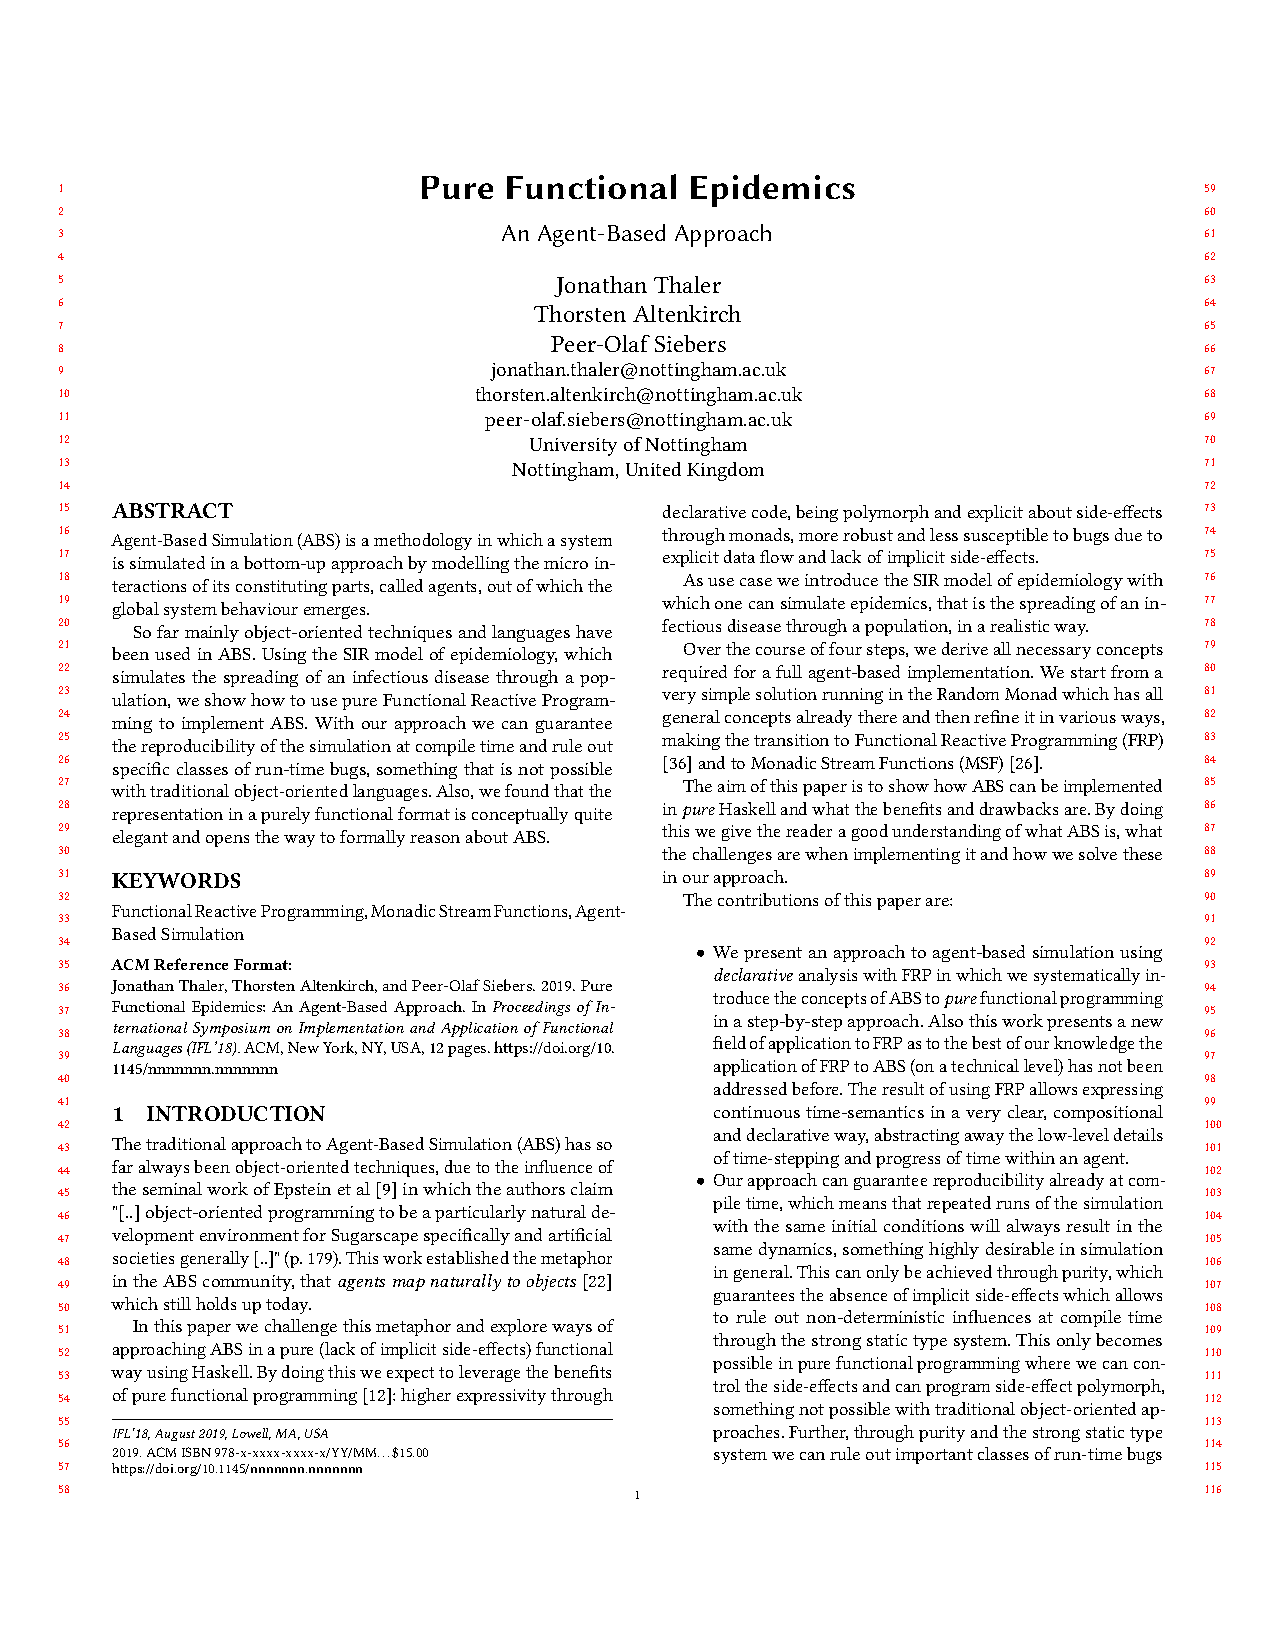
\includepdf[pages=-]{./pdf/pfe.pdf}

% NOTE: keep it out to the submission for the reviewers
%\chapter{Questions \& Answers}
\label{chap:qa}

TODO: update and adopt to 2nd year

In this chapter I give answers to anticipated questions and objections about my research direction and vision of doing pure functional ABS \footnote{They are not always posed in a dead-serious way but as it is a quite controversial topic - ABS should be done object-orientated after all huh? - I think it is appropriate. Also some objections were raised in exactly this way.}.

\paragraph{So you had this hypothesis, that pure functional programming and dependent types lead to simulation software which is more likely correct and is easier to verify and validate, right from the beginning?}
Not at all. I even had no deep knowledge of functional programming at the start of my PhD, I've just worked through the 1st edition of Grahams book "Programming in Haskell" and that's it. I had no clear understanding of purity, side-effects and Monads and I didn't know a bit about functional reactive programming. I knew that something like Dependent Types exist because Thorsten (2nd Supervisor) has sent me an email before the start of my PhD in which he pointed at Agda, so I started reading a bit about intuitionistic / constructivistic math, tried out a little bit of Agda but quickly gave up because it was way too far away (without really having mastered pure functional programming in Haskell, I believe it is nearly impossible / too difficult / makes no sense going into dependent types).
So in the beginning there was pure \textit{curiosity} about functional programming in combination with ABS because I knew nothing of FP at all and wanted to understand it (after getting bored by OO) and applying FP to ABS seemed so crazy (because everyone claims OO to be 'natural' for it) that it must be an extremely interesting challenge. I guess this is very often the case with research: there is 'just' curiosity in the beginning and then during the research process a hypothesis falls into place.


\chapter{Thesis Structure}
\label{app:thesis_struct}

TODO: find the story of my PhD thesis and connect it to my publication plan. 
TODO: story e.g. "We need functional programming to reduce the potential sources of bugs and introducing bugs harder, resulting in software which is more likely to be correct. Additionally by using dependent types we can narrow the gap between model specification and implementation even further, resulting in software which is even more likely to be correct. Further, additional benefits fall into place: purity leads to guaranteed reproducibility at compile-time, software transactional memory can be utilised to scale up to massively parallel and we have property-based testing at hand which puts the focus on specification testing rather than testing operational details".

This appendix gives a first draft of the structure outline of the thesis which I plan on start writing in April 2019. I aim for a flat structure which emphasises a strong narrative. The order of writing will be: Methodology, Proof-Of-Concept chapters, Literature Review, Discussion, Conclusions, Introduction, Abstract.
%
%line of argument
%1. established methods need extensive unit-testing for establishing correctness of software, which only increases the likelihood of correctness and doesnt guarantee it because they are inherent dynamic, testing run-time behaviour, because of the different type system.
%2. functional programming as in haskell has a strong static type system which allows to shift much much more guarantees towards static, compile-time, making many run-time tests obsolete and can guarantee a few things already at compile-time which makes tests to cover that completely obsolete
%3. dependent types can push these guarantees even further and theoretically should allow to express guarantees at compile-time to an arbitrary complex level which in theory should allow us to abandon run-time testing of bugs altogether. This does not mean that we don't need any tests anymore, as will be outlined in the chapter on Verification \& Validation \ref{chap:v_and_v}.
%4. with shifting more towards compile-time guarantees we automatically gain more confidence into the correctness of our simulation and reduce the implementation overhead of writing tests for those cases. Also some properties are simply not testable with run-time tests e.g. that some property holds forever - this is only possible to guarantee by looking at the code directly (where functional programming shines) or expressing it through compile-time guarantees. 
%5. correct by construction: narrowing the gap between model specification and implementation 
%6. Impedance Mismatch: ABS is constructive / generative in nature but the nature of the test-driven development process is deductive. is this a problem? Think of it more deeply


\section{Introduction}
This chapter is the introduction to the thesis and motivates it and describes the aim and scope of the Ph.D. Further it states the hypotheses and contributions.
\begin{itemize}
	\item Main Argument: Defining the problem, motivation, aim and scope of the Ph.D.
	\item Hypotheses: Precisely stating the hypotheses which will form the points of reference for the whole research.
	\item Contributions: Precisely list the contribution to knowledge this Ph.D. makes and list all papers which were written (and published) during this Ph.D.
\end{itemize}

\section{Literature Review}
This chapter discusses background and related work by presenting the relevant literature 

\section{Methodology}
This chapter introduces the methodology, used in the experimental chapters:

\begin{itemize}
	\item Defining and introducing Agent-Based Simulation (ABS) (History, ABS vs. MAS, examples, event- vs. time-driven).
	\item Introduce established implementation approaches to ABS (Frameworks: NetLogo, Anylogic, Libraries: RePast, DesmoJ, Programming: Java, Python, Correctness: ad-hoc, manual testing, test-driven development)
	\item Introduction Verification \& Validation (V \& V in the context of ABS).
	\item Introduction to functional Programming in Haskell (functions, types, recursion, algebraic data-types, higher-order functions, continuations, Define and explain side-effects and purity: monads, different types of effects, explain IO and that it is of fundamental importance to avoid it in our research).
	\item Introduction to dependent types (Example, Equality as Type, Philosophical Foundations: Constructive mathematics)
\end{itemize}

\section{Case Studies}
Presents case studies which are the main contribution of this Ph.D. which support our hypothesis. Each section is structured by Intro, Methods, Experiment, Analysis.

\subsection{Case Study 1: Testing and Verification}
This chapter describes how testing \& verification works in pure functional ABS.
%\begin{itemize}
%	\item Testing in functional programming
%	\item Strong Static Types rule out some classes of bugs and make some tests obsolete.
%	\item Property-Based testing: QuickCheck.
%	\item Using Property-Based testing in ABS for specification testing.
%	\item Reasoning about code
%\end{itemize}

\subsection{Case Study 2: Going Large-Scale}
This chapter discusses how pure functional ABS can go large-scale using STM. Further it is the central chapter, discussing various types of agent-agent and agent-environment interactions

%\subsubsection{Agent-Agent Interactions}
%This is the central problem of the FP approach as basically the agent-interactions define the level of abstractions over the agents. Unfortunately this is easier and more elegant in object-oriented programming. Still, by using a strong static type system we are more explicit about agent-interactions and we can have advantages which OOP doesn't have. Also we show that there are multiple different kinds of agent-interactions, depending on whether it is a time- or event-driven ABS.
%There is still much work to be done for this thesis chapter, we need to distinguish between:
%
%\begin{itemize}
%	\item Asynchronous Interaction: the flow is one-directional and does not need a listener on the other side and not a synchronous reply. The mechanism depends strongly on the type of ABS: time- or event-driven and pure or concurrent. Examples are the pure feedback in the Yampa SIR implementation, pure Data-Flow in the Yampa implementation, pure agent transactions, pure events, STM Event, STM message-boxes.
%	\item Synchronous Interactions: the flow is bi-directional and needs a listener on the other side to engage in a synchronous interaction without time-delay. We have only touched on prototyping this but need to go deeper for the final thesis. In Haskell we could build on the pure event driven approach we have implemented already in Step7\_EventDriven but we need to extend it towards an explicit synchronous mechanism. Also we need to show how we can do this in STM but there its gonna be very tricky because all agents act conceptually at the same time.
%\end{itemize}

\subsection{Case Study 3: Dependent Types}
This chapter gives an in-depth discussion on how dependent types can be made of use in pure functional ABS.

\section{Discussion}
This chapter re-visits the hypotheses and puts them into perspective of the contributions.

\section{Conclusions}
This chapter draws conclusions to the main hypothesis and outlines future research.

\section{Appendices}
Datasets, lengthy code, additional proofs.


\end{appendices}

\end{document}
